\documentclass{aastex63}
\usepackage{amsmath}
\newcommand{\be}{\begin{eqnarray}}
\newcommand{\ee}{\end{eqnarray}}
\def\la{\mathbin{\lower 3pt\hbox
      {$\rlap{\raise 5pt\hbox{$\char'074$}}\mathchar"7218$}}}
\def\ga{\mathbin{\lower 3pt\hbox
      {$\rlap{\raise 5pt\hbox{$\char'076$}}\mathchar"7218$}}} %> or of order
\renewcommand{\vec}[1]{\mathbf{#1}}
%\renewcommand{\vec}[1]{\ensuremath{\boldsymbol{#1}}} %boldface vector style
\newcommand{\grad}{\mathbf{\nabla}}
\newcommand\lya{Ly$\alpha$\ }


\received{}
\revised{}
\accepted{\today}
\submitjournal{APJ}


\shorttitle{Resonant Scattering of \lya}
\shortauthors{McClellan et al.}

\graphicspath{{./}{figures/}}


\begin{document}

\title{Resonant Scattering in a Uniform Sphere with Large Optical Depth}



\correspondingauthor{B. Connor McClellan}
\email{bcm2vn@virginia.edu}

\author{B. Connor McClellan}
\author{Shane Davis}
\author{Phil Arras}
\affiliation{Department of Astronomy, University of Virginia, Charlottesville, VA 22904, USA}


\begin{abstract}

The solution of the radiative transfer equation for resonant scattering of Lyman $\alpha$ photons is explored in spherical geometry. A monochromatic source of photons is assumed at the center of a uniform sphere of constant gas density. The intensity within the sphere and at its surface is found in the limit of large line-center optical depth using the Eddington approximation for the angular dependence. Two specific problems are studied: a steady source and an impulsive source. For the steady-state problem, the solution can be represented as a sum of two terms: a previously-known analytic solution of the homogeneous equation with the mean intensity $J=0$ at the surface, and a novel, semi-analytic solution of the homogeneous equation which enforces the correct, zero-ingoing intensity boundary conditions at the surface. This solution is compared to that of the Monte-Carlo method, which is valid at arbitrary optical depth. It is shown that the size of corrective term depends on the line center optical depth, and may explain discrepancies in previous studies that used a $J=0$ boundary condition. For the impulsive problem, the time dependence, spatial dependence, and photon frequency dependence of the diffusion equation is expressed using an eigenfunction expansion and solved numerically to characterize the escape time distribution and spectra of photons initialized at the center of the sphere. It is shown that the lowest-order eigenfrequency of the semi-analytic calculation agrees well with the decay constant of the Monte Carlo escape time distribution at line-center optical depths above ${\sim} 10^7$. A fitting function for the distribution is found which can be sampled to accelerate Monte Carlo radiation transfer calculations at very large optical depths.

\end{abstract}


\keywords{}

\section{Introduction}
\label{sec:intro}

The outer layers of planetary atmospheres are central to a planet's evolution, since they can shelter the lower atmosphere from high energy radiation as well as regulate the escape of gas into space. Ionization and subsequent recombination can generate \lya within the planet's atmosphere, dissociating molecules in lower layers and creating pressure forces that drive an outflow of escaping H atoms. \lya can also excite H atoms to the 2p state, creating a population of Balmer-line absorbers that can be observed via transmission spectroscopy \citep{2017ApJ...851..150H}.

Hubble Space Telescope (HST) observations with the STIS have found large \lya transit depths around a handful of exoplanets \citep{2003Natur.422..143V, 2012A&A...543L...4L, 2012A&A...547A..18E, 2015Natur.522..459E,  2017A&A...597A..26B, 2017A&A...599L...3B, 2017A&A...602A.106B, 2018A&A...620A.147B, 2019AJ....158...50W, 2019EPSC...13.1928L, 2020ApJ...888L..21G,2021arXiv210309864B}. These observations have revealed a population of atoms extending out to distances of order a few planetary radii for several planets around bright, nearby stars, motivating a study of the physics of \lya interactions with the H atom population. In atmospheres with thick layers of atomic hydrogen, stellar Lyman Alpha (Ly$\alpha$) radiation is especially important in the atmospheric dynamics of these systems as the optical depth at line center is large. The importance of the \lya line in this process necessitates a careful treatment of resonant scattering in order to construct accurate models of H atom excitation, heating, and radiative forces. 

Numerical simulations can be used to understand the complex layers of these irradiated exoplanet atmospheres. However, the extreme optical depths at \lya line center introduce a computational barrier to simulating radiative transfer via Monte Carlo methods. The main impediment to performing magnetohydrodynamic simulations with fully a coupled radiative transfer solution via Monte Carlo methods is the prohibitive computational cost. The number of scatterings a photon undergoes is proportional to the line center optical depth.  Near the base of the atmosphere, the line center optical depth is ${\sim}10^9$, so most of the time is spent following photons in these cells. A method that can treat these zones via a simple solution rather than Monte Carlo has the potential to greatly accelerate the calculation. A complete, general analytic solution for the resonance scattering has never been derived but approximate solutions exist in certain limits.

\citet{1973MNRAS.162...43H} demonstrated in slab geometry that resonance-line radiation transfer in optically-thick media can be described by the Poisson equation. However, their solution contains an incorrect treatment of the boundary condition. To our knowledge, the errors introduced by this treatment have never been quantified. They attempt a separation of variables $J(\tau,\sigma) = \theta(\tau) j(\sigma)$ in spatial variable $\tau$ and frequency variable $\sigma$ (their Equations 16 and 23). The solutions for the eigenfunctions $\theta(\tau)$ and $j(\sigma)$ then depend explicitly on the separation constant $\lambda$. In order to satisfy the boundary conditions, the separation constant must satisfy an eigenvalue equation of the form
\be
\lambda \tan(\lambda B) & = & \frac{3}{2} \phi \Delta,
\label{eq:evalue}
\ee
where $2B$ is the slab optical depth at line center, and $\phi$ is the line profile. The key point is that the line profile depends on one of the coordinates, frequency, and this causes the eigenvalues of the separation constant to depend on frequency. Thus, the separation constant is not constant, and it does not satisfy the Poisson equation since the frequency derivatives will act on the separation ``constant", giving extra terms. In the limit of large optical depth $B$, they approximate the eigenvalues as $\lambda_n B \simeq \pi (n-1/2)$. However, this solution gives zero mean intensity at the surface. Their Eq. 34 subsequently allowed the separation constant to have a small deviation from the above expression, which was explicitly frequency dependent. This allowed a nonzero intensity at the surface, but at the cost of rendering the separation of variables assumption invalid. Our treatment, using the correct boundary condition, quantifies the errors in their ansatz.

Several other works have followed \citet{1973MNRAS.162...43H}, building upon their result without addressing the incorrect boundary condition. \citet{1990ApJ...350..216N} attempts to extend the solution to media of intermediate optical depth, including the effects of scattering in the Doppler core of the line, but again does not use the correct boundary condition. \citet{2006ApJ...649...14D} generalize the same problem to spherical geometry, as is used here. Following this, \citet{2015MNRAS.449.4336S} employ a ``core skipping'' method to handle photon frequency redistribution within the Doppler core. This technique involves drawing the atom's velocity from a truncated Gaussian distribution, forcing photons back into the wing when they scatter into the core. % This is motivated by the assumption that all core scattering results in zero spatial diffusion until the photon is redistributed back out into the wing where the mean free path becomes much larger and it can diffuse in space again. However, it is not clear whether this prescription is fully independent of the choice of velocity distribution. 

\section{STEADY-STATE SOLUTION}
\label{sec:steadystate}

Consider a sphere of radius $R$ and uniform density, with line-center optical depth $\tau_0$. We aim to find the intensity within the sphere as a function of radius and photon frequency. Photons of frequency $\nu$ near line center frequency $\nu_0$ are considered. The Doppler width will be written $\Delta = \nu_0 v_{\rm th}/c$, where $v_{\rm th}=\sqrt{2k_{\rm B}T/m_{\rm H}}$ is the thermal speed of hydrogen atoms of mass $m_{\rm H}$ and temperature $T$, and $c$ is the speed of light. The photon frequency in Doppler units will be written $x = (\nu-\nu_0)/\Delta$. For upper-state de-excitation rate $\Gamma$, the ratio of natural to Doppler broadening is $a=\Gamma/(4\pi \Delta)$. $n_{\rm sc}$ is the number density of scatterers, $e$ and $m_e$ are the charge and mass of the electron, $f$ is the oscillator strength of the transition, $\mathcal{H}(x,a)$ is the Voigt function, $k = n_{\rm sc} (\pi e^2/m_e c) f$, and the Voigt line profile is $\phi = \mathcal{H}(x,a)/(\sqrt{\pi} \Delta)$, which is normalized as $\int d\nu\, \phi(\nu) = 1$. The line center optical depth is then $\tau_0 = (k/\sqrt{\pi}\Delta)R$. 

Starting with the full transfer equation, Eq. \ref{app:rteqn_derivation}\ref{eq:finaleqn}, with no photon destruction and a photon emission term given by Eq. \ref{app:rteqn_derivation}\ref{eq:jem}, the steady-state transfer equation is
\be
\nabla^2 J + \left( \frac{k}{\Delta} \right)^2 \frac{\partial^2 J}{\partial \sigma^2} & = & 
- \frac{ \sqrt{6} kL}{4\pi \Delta^2} \delta^3(\vec{x} - \vec{x}_s) \delta (\sigma - \sigma_{\rm s}).
\label{eq:rt_no_destr}
\ee
where $\sigma$ comes from a change of variables in photon frequency (Eq. \ref{app:rteqn_derivation}\ref{eq:change_of_variables}) and $\sigma_s$ is the photon frequency of the source. The boundary condition is that there is no incoming intensity at the surface, which can be written
\citep{1986rpa..book.....R}
\be
J & = & \sqrt{3} H
\label{eq:bc}
\ee
at $r=R$. 

A solution for the mean intensity $J_d$ which is divergent at the center of the coordinate system and at the emission frequency is presented in \citet{1990ApJ...350..216N}. Here it is extended to spherical geometry and generalized to allow emission frequencies away from line center: 
\be
J_{\rm d} & = & 
\left(\frac{\sqrt{6}k^2L}{16\pi^3 \Delta^3}\right)\left(\frac{1}{(kr/\Delta)^2 + (\sigma - \sigma_{\rm s})^2}\right)
\label{eq:Jd}
\ee

\be
H_{\rm d} & = & - \frac{1}{3k\phi} \frac{\partial J_d}{\partial r}
=  \left( \frac{1}{3k\phi} \right) 
\left( \frac{ \sqrt{6}k^3L }{ 8\pi^3 \Delta^4} \right)
\left( \frac{k r/\Delta}{ \left[ (kr/\Delta)^2 + (\sigma-\sigma_{\rm s})^2 \right]^2 } \right).
\label{eq:Hd}
\ee
This solution is useful as a very simple analytic formula. However, it is not a good approximation to the true solution, as it is too large at $r=R$ by a factor of $J_{\rm d}(R,\sigma)/ H_{\rm d}(R,\sigma) \sim a\tau_0/x^2 \sim (a\tau_0)^{1/3} \gg 1$ and does not adhere to the correct boundary condition. This solution is included in Fig. \ref{fig:sol_mc_residual_0} for illustration, but will not be discussed further.

A better approximation to the true solution has been derived by \citet{2006ApJ...649...14D}, who generalized the closed-form solution in slab geometry found in \citet{1990ApJ...350..216N}. They found a solution which satisfies a $J=0$ boundary condition at $r=R$. Again, we generalize their solution to allow emission at frequency $\sigma_{\rm s}$ away from line center. The result can be written as a sum over spatial modes,
\be \label{eq:J0_sum}
J_0 = \frac{\sqrt{6}L}{16\pi \Delta} \frac{1}{R^2}\sum_{n=1}^{\infty}n\frac{\sin{\kappa_n r}}{\kappa_n r}\exp{\left(\frac{\kappa_n \Delta}{k}|\sigma - \sigma_s|\right)},
\ee
and
\be \label{eq:H0_sum}
H_0 = - \frac{1}{3k\phi} \frac{\partial J_0}{\partial r} = -\frac{1}{3k\phi}\frac{\sqrt{6}L}{16\pi\Delta} \frac{1}{R^2}\sum_{n=1}^{\infty}n\left(\frac{\cos{\kappa_n r}}{r} - \frac{\sin{\kappa_n r}}{\kappa_n r^2}\right)\exp{\left(\frac{\kappa_n \Delta}{k}|\sigma - \sigma_s|\right)},
\ee
which can be summed to give the closed form expressions
\be
J_0 & = & \frac{\sqrt{6}L}{32\pi^2 \Delta}
\frac{1}{Rr}
\left( 
\frac{ \sin(\pi r/R) }{ \cosh \left[ \frac{\pi \Delta}{k R} (\sigma - \sigma_{\rm s}) \right] - \cos(\pi r/R)}
\right)
\label{eq:J0}
\ee
and
\be
H_0 & = &\frac{1}{3k\phi}
\frac{\sqrt{6}L}{32\pi^2 \Delta}
\frac{1}{Rr^2}
\left( 
\frac{ \sin(\pi r/R) }{ \cosh \left[ \frac{\pi \Delta}{k R} (\sigma - \sigma_{\rm s}) \right] - \cos(\pi r/R)}
\right. \nonumber \\ & & \left. - \left( \frac{\pi r}{R} \right)
\frac{ \cos(\pi r/R) }{ \cosh \left[ \frac{\pi \Delta}{k R} (\sigma - \sigma_{\rm s}) \right] - \cos(\pi r/R)}
+ \left( \frac{\pi r}{R} \right)
\frac{ \sin^2(\pi r/R) }{ \left[ \cosh \left[ \frac{\pi \Delta}{k R} (\sigma - \sigma_{\rm s}) \right] - \cos(\pi r/R) \right]^2 }
\right).
\label{eq:H0}
\ee
Again $J_0 \gg H_0$, except very near the $r=R$, where it goes to zero. The flux at $r=R$ can be written
\be
\nonumber
H_0(R, \sigma) & = & - \frac{1}{3k\phi}
\frac{\sqrt{6}L}{16\pi \Delta}
\frac{1}{R^3}
\sum_{n=1}^{\infty} 
n (-1)^n \exp{\left(\frac{\kappa_n \Delta}{k}|\sigma - \sigma_s|\right)}\\
& = &  \frac{1}{3k\phi}
\frac{\sqrt{6}L}{32\pi \Delta}
\frac{1}{R^3}
\left( 
\frac{ 1 }{ \cosh \left[ \frac{\pi \Delta}{k R} (\sigma - \sigma_{\rm s}) \right] +1 }
\right).
\label{eq:H0surf}
\ee
Eq. \ref{eq:H0surf} will be shown to be a much better approximation to the solution than Eq. \ref{eq:Hd}. It is still valid near the delta function at $r=0$, but is also a much better approximation at $r=R$. $J_0$ decreases exponentially rather than as a power-law in frequency as for $J_d$, giving a much smaller flux on the line wings as compared to the divergent solution. 

 %TODO

A different solution method is attempted here, namely, a continuous Fourier expansion in the frequency variable $\sigma$. The solution of this problem is split into two pieces: $J_0$ which includes the delta function source and satisfies $J=0$ at $r=R$, and $\rm J_{bc}$ which allows the boundary condition $J=\sqrt{3}H$ to be satisfied. The total solution is
\be
J(r,\sigma) & = & J_0(r,\sigma) + J_{\rm bc}(r,\sigma)
\ee
and
\be \label{eq:totalflux}
H(r,\sigma) & = & H_0(r,\sigma) + H_{\rm bc}(r,\sigma).
\ee
Here, $J_0$ and $H_0$ are the solutions of the homogeneous equation, given in Equations \ref{eq:J0} and \ref{eq:H0}. The additional term $J_{\rm bc}$ must then be a solution of the homogeneous equation
\be \label{eq:diffeq}
\frac{\partial^2J_{\rm bc}}{\partial r^2} + \frac{2}{r} \frac{\partial J_{\rm bc}}{\partial r}
+ \left( \frac{k}{\Delta} \right)^2 \frac{\partial^2 J_{\rm bc}}{\partial \sigma^2} &= & 0
\ee
with no delta function source term, and it must allow the boundary conditions to be satisfied at the surface. Since $J_0(R,
\sigma)=0$, the surface boundary condition becomes
\be
J_{\rm bc}(R,\sigma) - \sqrt{3} H_{\rm bc}(R,\sigma) & = 
\sqrt{3} H_0(R,\sigma).
\label{eq:bc2}
\ee
Plugging in a frequency dependence $J_{\rm bc} \propto e^{is\sigma}$, for ``wavenumber" $s$, gives the equation for modified spherical Bessel functions of the first kind, $i_0(z)=\sinh(z)/z$. The solution can then be represented as
\be
J_{\rm bc}(r,\sigma) & = & 
\int_{-\infty}^\infty \frac{ds}{2\pi} e^{is\sigma} A(s) 
\frac{i_0(krs/\Delta)}{i_0(kRs/\Delta)},
\label{eq:Jbc}
\ee
where $A(s)$ is the Fourier amplitude. Plugging Eq. \ref{eq:Jbc} into Eq. \ref{eq:bc2} leads to the following equation for the Fourier amplitudes,
\be
\int_{-\infty}^\infty \frac{ds}{2\pi} e^{is\sigma} A(s)
\left[ 1 + \left( \frac{s}{\sqrt{3} \Delta \phi} \right) \left( \frac{i_0^\prime(kRs/\Delta)}{i_0(kRs/\Delta)} \right) \right]
& = & \sqrt{3} H_0(R,\sigma)
\label{eq:bc3}
\ee
where $H_0(R,\sigma)$ is given by Eq. \ref{eq:H0surf}. Discretization of Eq. \ref{eq:bc3} for frequency variables $\sigma_i$ and wavenumbers $s_j$
leads to a set of coupled linear equations for the $A(s_j)$. We use equally-spaced points $\Delta \sigma = 2\sigma_{\rm max}/(N-1)$ and $\Delta s = 2\pi/(N\Delta \sigma)$, where $N$ is the number of points for each grid. The result is a linear system to solve for the $A(s)$. The maximum frequency is set as $\sigma_{\rm max} = {\rm constant} \times \tau_0$, for a large enough constant that  the end of the frequency grid is at such small intensities that it does not affect the solution except close to the boundaries. The number of points was increased until the solution was well-resolved near line center, and only became inaccurate very near the boundaries. Given the Fourier amplitudes, $J_{\rm bc}$ is computed using Eq. \ref{eq:Jbc}, and the flux is given by
\be
H_{\rm bc}(r,\sigma) & = & \left( \frac{-1}{3k\phi} \right)
\frac{\partial J_{\rm bc}(r,\sigma)}{\partial r}
= \left( \frac{-1}{3k\phi} \right)
\int_{-\infty}^\infty \frac{ds}{2\pi} e^{is\sigma} A(s) 
\left( \frac{ks}{\Delta} \right) 
\left( \frac{i_0^\prime(krs/\Delta)}{i_0(kRs/\Delta)} \right).
\label{eq:Hbc}
\ee
The Bessel functions are finite at the center and rise steeply toward the surface when $kRs/\Delta \gg 1$. 

\subsection{Scaling with Line Center Optical Depth}
To examine the relative size of the correction term $H_{\rm bc}$ as compared to $H_0$, we consider the case where the $\tau_0$ is large and thus $J_{\rm bc} \gg H_{\rm bc}$. We obtain the proportionality
\be \label{eq:hbc_scaling}
\frac{H_{\rm bc}(R, \sigma)}{H_0(R, \sigma)} \propto \frac{1}{(a\tau_0)^{1/3}}.
\ee
Thus, the fractional importance of the correct frequency-dependent boundary condition term $H_{\rm bc}$ scales as $(a\tau_0)^{-1/3}$. At very large $\tau_0$, it is expected that the correction term will be small, but will become increasingly important as $\tau_0$ decreases.

The location of the spectral peak of the distribution is
\be \label{eq:tau_peak_scaling}
x_{\rm peak} {\sim} \left(a\tau_0\right)^{1/3}.
\ee
The solutions of the transfer equation will perform best when the peaks of the spectral energy distribution lie well outside of the Doppler core, e.g., for large $\tau_0$. For \lya and H atoms with $T=10^4$ K, the damping parameter is $a = \Gamma / (4\pi\Delta) = 4.72\times 10^{-4}$. Thus, the value of $x$ at which the Doppler and Lorentzian components of the line wing are equal is $x_{\rm cw}=3.3$. Setting $x_{\rm cw} = x_{\rm peak}$ and solving for $\tau_0$ gives the value of the line-center optical depth at which the core of the line moves into the peak of the spectrum, which is $\tau_{\rm cp}=7.3\times10^4$. Solutions derived assuming a Lorentzian line profile $\phi(x) \approx a/(\pi x^2)$ are expected to fail for lower line center optical depths where the peak of the spectrum lies near the core and improve for larger optical depths where the spectral peak is well outside of the line core.

\subsection{Comparison to Monte Carlo}
The Monte Carlo method is used to solve the transfer equation numerically. This method is valid at arbitrarily large optical depths, being restricted only by its computational demand which grows proportionally to the number of photons used and $\tau_0$. For each simulation, a total of ${\sim}10^6$ photon packets are initialized at a monochromatic source frequency $x_s$ and are allowed to propagate through the sphere until escaping, at which point their positions, outgoing angles, and escape frequencies are stored. A constant temperature of $T=10,000\ \rm K$ is set for the gas. Frequency redistribution is calculated at each scattering, including the effects of recoil, to obtain the spectrum at the surface of the spherical simulation domain. In the comparisons shown in this section, the raw photon data is binned in frequency to obtain spectra. 64 bins are used to ensure good statistics and minimal noise in each bin. Further details of the Monte Carlo implementation are discussed in \cite{2017ApJ...851..150H}.

\ifx
\begin{figure}
    \centering
    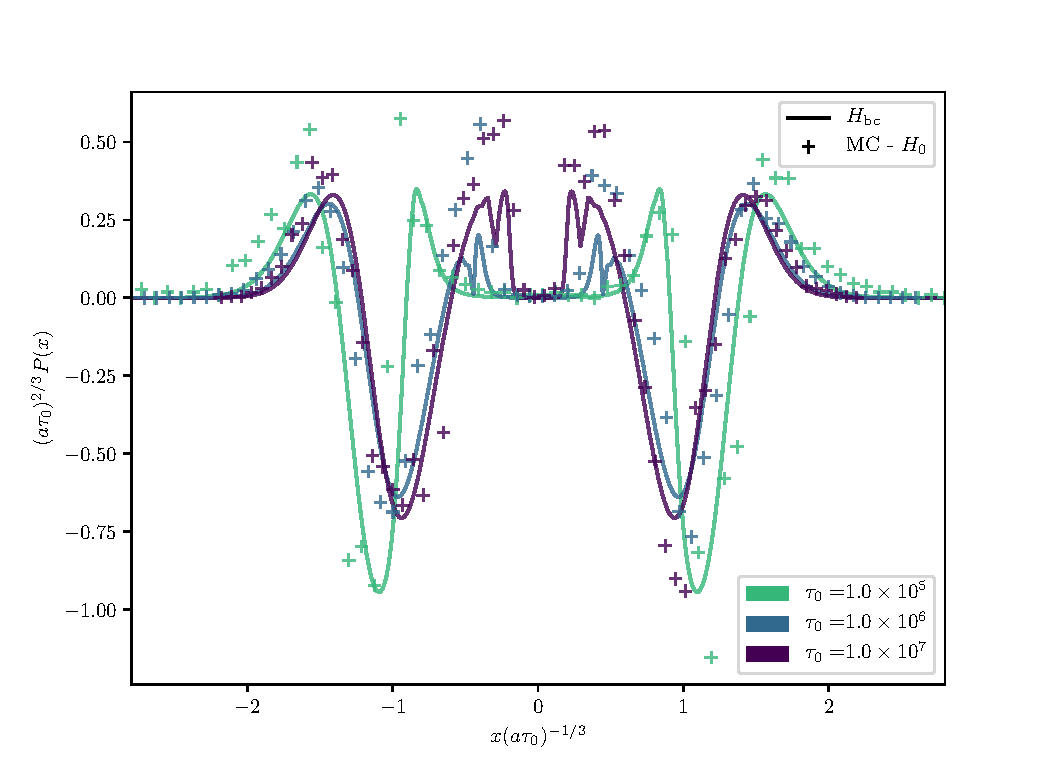
\includegraphics{taubc.pdf}
    \caption{Boundary condition term $H_{\rm bc}$ scaled by $(a\tau_0)^{1/3}$ shown for increasing line center optical depths. The Monte Carlo data minus the $H_0$ solution should be close to $H_{\rm bc}$ according to Eq. \ref{eq:totalflux}. As $\tau_0$ becomes larger, the agreement between these two improves, indicating that at large optical depths the relative size of the corrective boundary condition term scales as $(a\tau_0)^{-1/3}$}.
    \label{fig:taubc}
\end{figure}
\fi

\begin{figure}
    \centering
    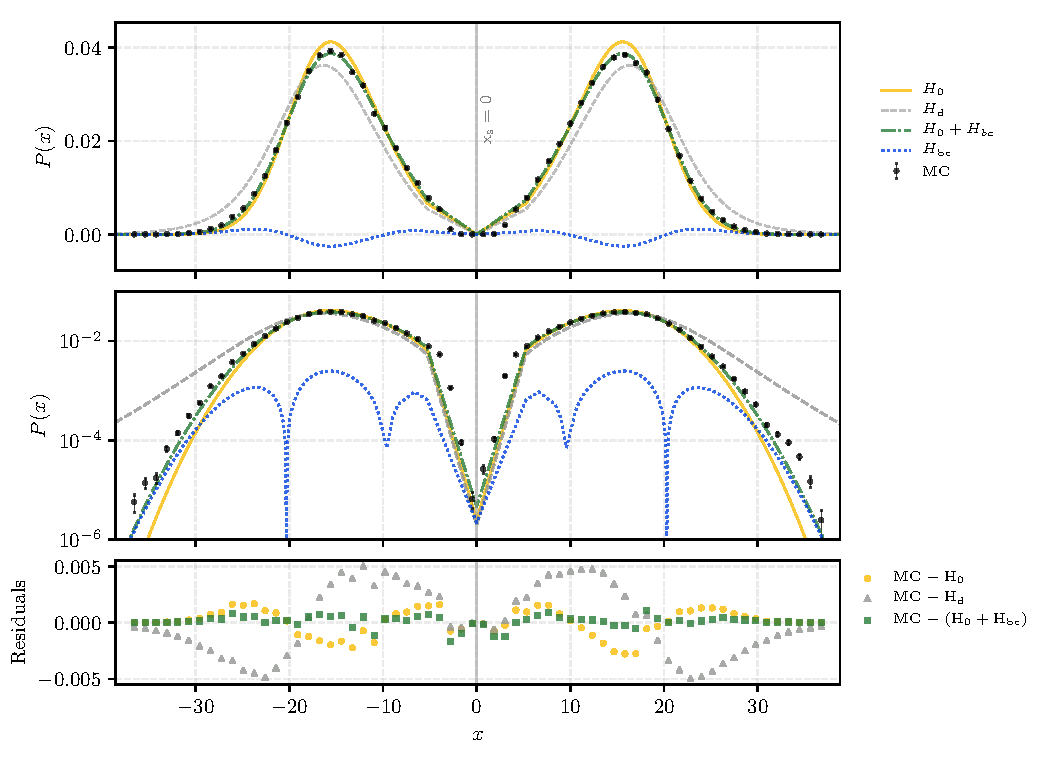
\includegraphics{final_residual.pdf}
    \caption{Analytic solution for the outgoing spectrum compared with Monte Carlo at a line center optical depth of $\tau_0 = 1 \times 10^7$. Photons are initialized with $\rm x = 0.0$. In the log-scale plot in the second panel, $|\rm H_{bc}|$ is shown instead of $\rm H_{bc}$ to examine the contributions of both positive and negative pieces. Residuals of each solution to the Monte Carlo data points are shown in the third panel.} 
    \label{fig:sol_mc_residual_0}
\end{figure}

We now compare each of the previously-discussed solutions for surface flux with Monte Carlo simulations. We return to the Doppler units $x$ for the photon frequency rather than the $\sigma$ units used in the solutions of the transfer equation. The spectrum $P(x)$ is defined as the specific luminosity at the surface divided by the source luminosity, or
\be
P(x) = \frac{16\pi^2R^2H(R, x)\Delta}{L}.
\ee
This is normalized such that $\int P(x)dx = 1$. Since $H(r, x)$ is per $d\nu$, a factor of $\Delta$ gives the expression the correct units. 

% TODO: Edits unclear. Organization of sentences OK? "Describe what's in the figure and then discuss" - Mention of Hd moved to end of paragraph, details of the Hbc term moved higher up.
In Figure \ref{fig:sol_mc_residual_0}, the Monte Carlo escape probability as a function of frequency is shown with that of the solutions $H_{\rm d}$, $H_{\rm 0}$, and $H_{\rm 0 + bc} = H_{\rm 0} + H_{\rm bc}$ for an optical depth of $\tau_0 = 10^7$ and photons emitted at line center $\rm x_s = 0$.  The $H_{\rm bc}$ term is negative at the peak of the spectrum and positive in the line wing such that, when added to the solution $H_0$ derived by \citet{2006ApJ...649...14D}, it adequately corrects for the apparent excess of flux in the peaks of the spectrum. This peak excess is also present in previous work that used the \citet{1990ApJ...350..216N} solution, such as \citet{2015MNRAS.449.4336S} where the discrepancy is particularly noticeable for line center optical depths of $\tau_0=10^5$ and $10^6$ in the top panel of their Figure 5. The solution with the correct frequency-dependent boundary condition enforced, $H_{\rm 0 + bc}$, has considerably lower residuals to Monte Carlo than the other solutions, especially in the line wing. The boundary term corrects the slight deficit of $H_{\rm0}$ in the line wings, further improving agreement with the numerical result. Note that the residuals to the $H_0$ solution are a close match to the $H_{\rm bc}$ term, since the Monte Carlo represents the ``true'' solution, $H$, and $H_{\rm bc} = H - H_0$. It is evident that the divergent solution $H_{\rm d}$ fails in the line wings.

 \begin{figure}
    \centering
    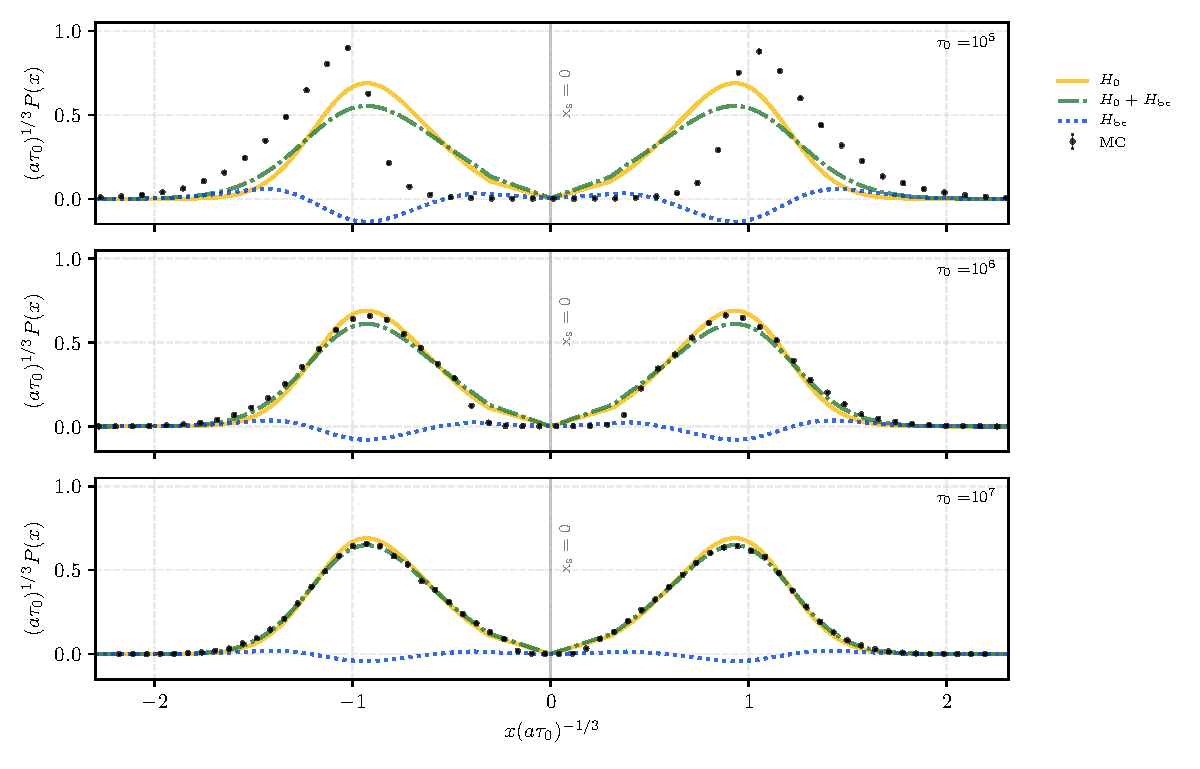
\includegraphics{tau_threepanel.pdf}
    \caption{The same as Figure \ref{fig:sol_mc_residual_0}, but for $\tau_0 = 10^5, 10^6, 10^7$. The $x$ and $y$ axes are scaled by $(a\tau_0)^{1/3}$. Photons are initialized with $\rm x_s = 0.0$ in each case.} 
    \label{fig:sol_mc_tau}
\end{figure}

The size of $H_{\rm bc}$ is dependent on $\tau_0$, which also dictates the x-position of the peak of spectrum according to Eq. \ref{eq:tau_peak_scaling}. This term is significant even at $\tau_0 {\sim} 10^7$ where $H_0$ solution is expected to perform its best, i.e., photons are pushed further out into the wing and thus the simplifying assumptions made in the solution of the differential equation are a better approximation. 

In Figure \ref{fig:sol_mc_tau} we show the solutions alongside Monte Carlo for $\tau_0=10^5, 10^6$, and $10^7$. From Eq. \ref{eq:hbc_scaling}, the size of the term $H_{\rm bc}$ should become smaller with larger optical depths, following a $(a\tau_0)^{-1/3}$ scaling. Indeed, agreement between Eq. \ref{eq:H0surf} and the Monte Carlo points in Fig. \ref{fig:sol_mc_tau} improves as $\tau_0$ increases, with $H_{\rm bc}$ providing a fractionally smaller correction to $H_0$. One factor of $(a\tau_0)^{1/3}$ has been scaled out of the x-axis such that the peaks of the distributions are vertically aligned. This scaling has also been applied to the y-axis to preserve normalization of the escape probability. At lower $\tau_0$, the scattering of photons within the Doppler core of the line becomes important, yet our solution does not include this effect. The effects of line core scattering can be seen in the Monte Carlo data, however, as the peaks of the distribution shift substantially outward in frequency from the line core for $\tau_0 = 10^5$.
 
 \begin{figure}
    \centering
    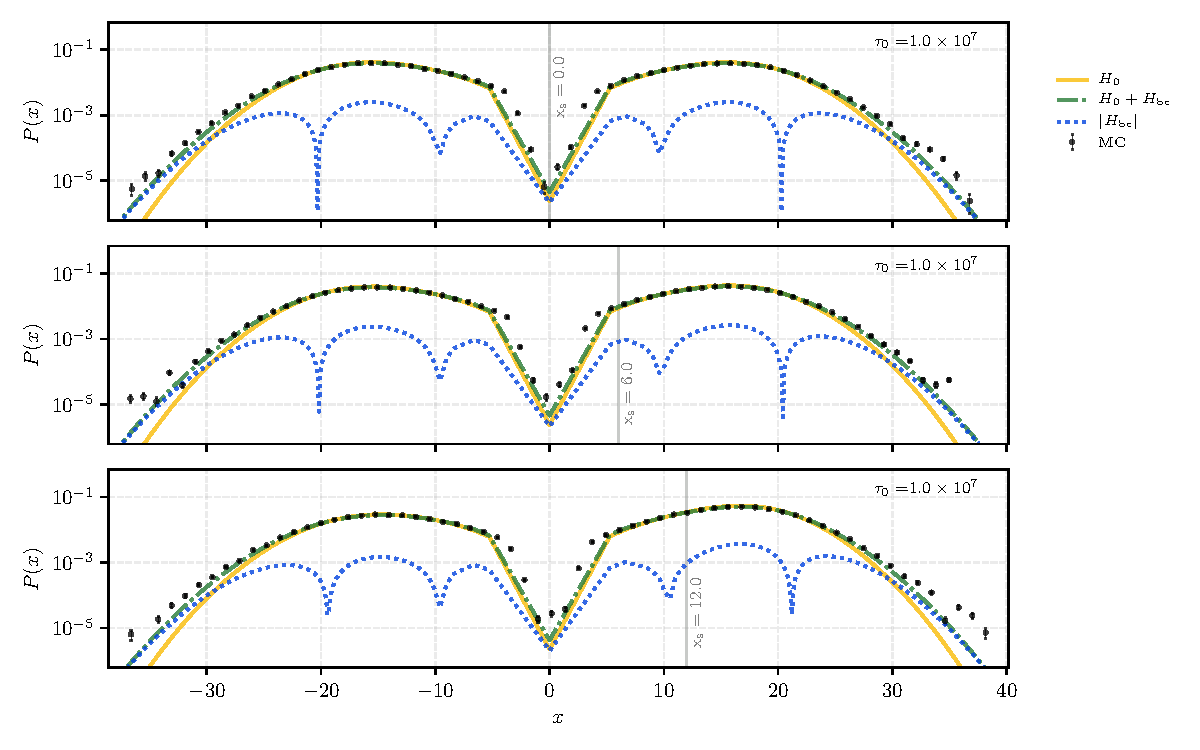
\includegraphics{xinit_threepanel.pdf}
    \caption{Analytic solution for the outgoing spectrum compared with Monte Carlo at a line center optical depth of $\tau_0 = 1 \times 10^7$. Photons are initialized with $\rm x = 0.0, 6.0, 12.0$ to examine the solutions' accuracy with a changing source frequency. The optical depth at each of these source frequencies is $\tau_s = 10^7, 77,$ and $19$, respectively.} 
    \label{fig:sol_mc_xinit}
\end{figure}

 \begin{figure}
    \centering
    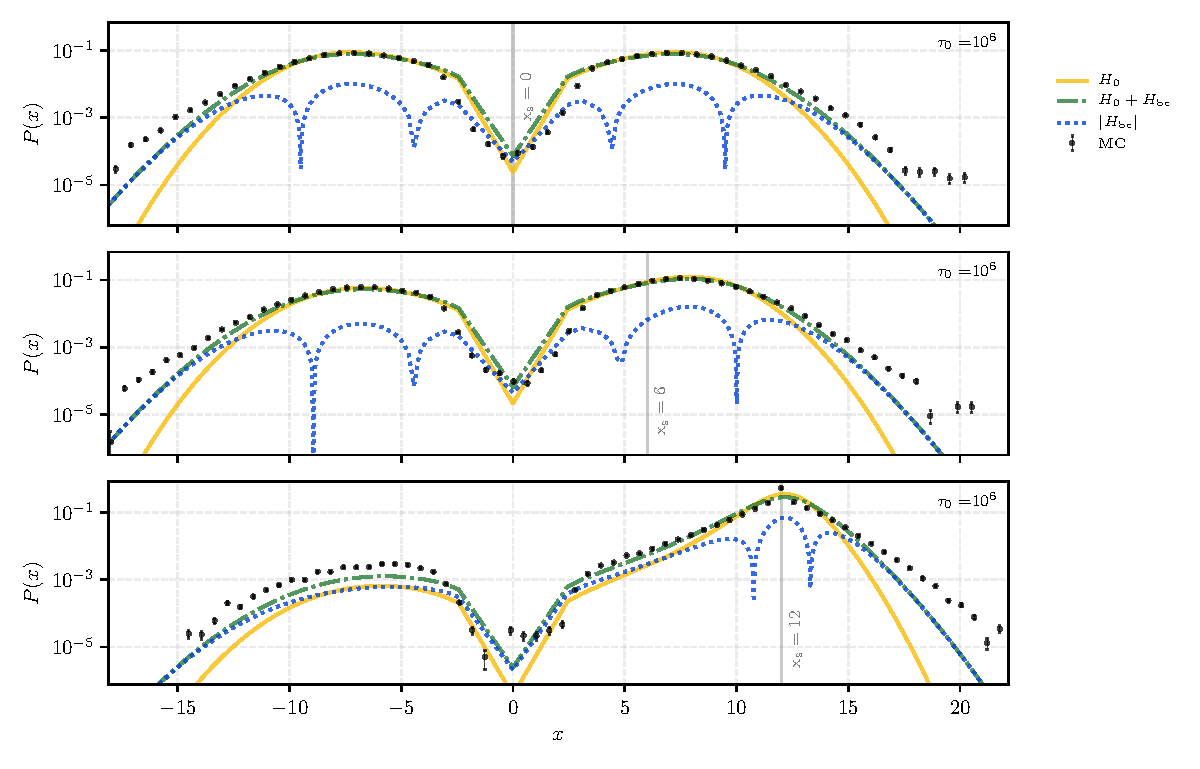
\includegraphics{xinit_threepanel_tau1e6.pdf}
    \caption{Again changing $x_s$, but at a lower optical depth of $\tau_0 = 10^6$. The shift in $x$ is a much larger fraction of the distance to the spectral peak $(a\tau_0)^{1/3}$, and thus the bias in the spectrum is much more drastic. The optical depth at the source frequency is $\tau_s = 10^6$, $7.7$, and $1.9$ for $x_s=0.0, 6.0,$ and $12.0$, respectively. } 
    \label{fig:sol_mc_xinit_lowtau}
\end{figure}

Since the solutions have been generalized to allow for a monochromatic source of photons at a frequency $x_s \neq 0$, their agreement with Monte Carlo as a function of source frequency can also be characterized. Photons initialized further out in the line wing have larger mean free paths. The larger spatial diffusion contributes to greater escape probability for these photons. In the limit that $|\rm x_s|$ becomes large, the distribution becomes a delta function in frequency as all photons escape the gas without scattering. 

Figure \ref{fig:sol_mc_xinit} shows calculations performed for three initial photon frequencies $\rm x_s = 0.0, 6.0$, and $12.0$ for a line center optical depth of $\tau_0=10^7$. The asymmetry of the spectrum is slight for $\rm x_s = 6.0$ where the cross section is still relatively large, but the increase in mean free path is much more substantial when photons are initialized with $\rm x_s=12.0$, further away from the line core. It is seen here that the difference between the Monte Carlo data and $H_0$ becomes larger as $\rm x_s$ increases. Thus, for sufficiently large $\tau_0$ and emission away from line center ($x_s \neq 0$), the importance of enforcing frequency-dependent boundary conditions at the surface of the sphere grows. 

Figure \ref{fig:sol_mc_xinit_lowtau} shows emission away from line center at the same values of $x_s$ as in Figure \ref{fig:sol_mc_xinit}, but for $\tau_0=10^6$ rather than $10^7$. The difference between the left and right side of the escaping spectrum is substantial at lower optical depths, since a change in $x_s$ of 6 is a larger fraction of the spectral peak location $(a\tau_0)^{1/3}$ for lower $\tau_0$. It is clear from the figure that as $x_s$ becomes further from the line core, the spectrum approaches a delta function in frequency. Additionally, since the material is optically thin here, we expect there to be a stronger disagreement between the Monte Carlo and the analytic solution as derivations assumed large optical depths.

\begin{figure}
    \centering
    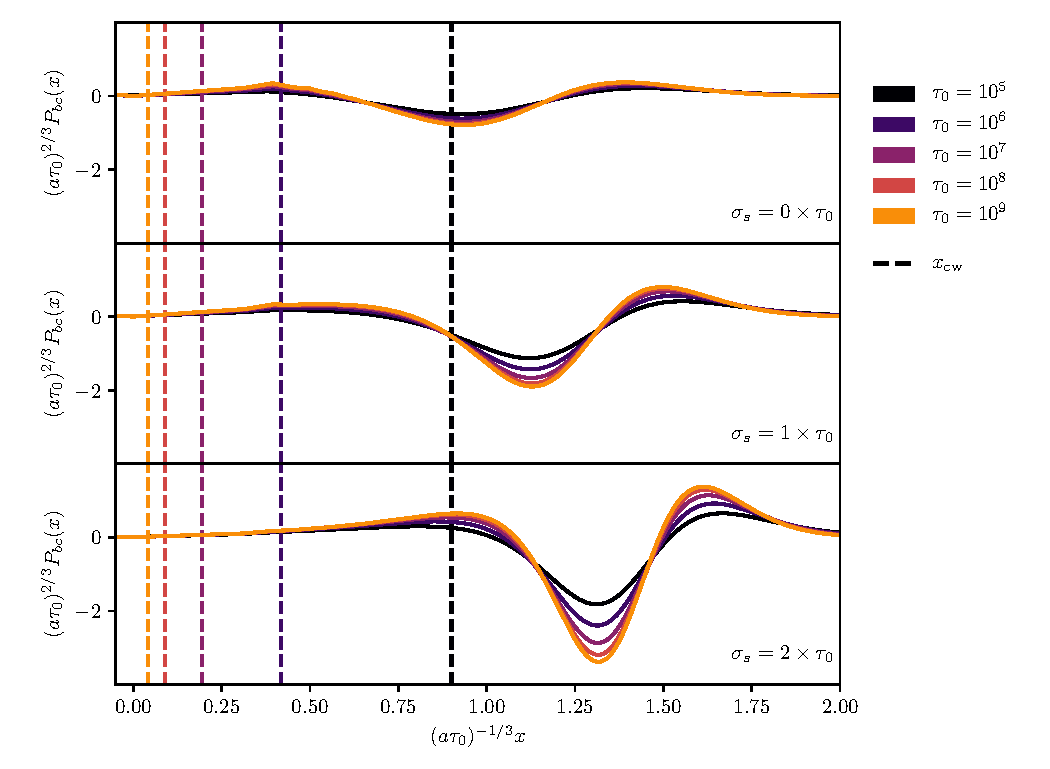
\includegraphics[width=\textwidth]{xinit.pdf}
    \caption{$H_{\rm bc}$ solutions shown at three line center optical depths, $\tau_0=10^5, 10^7,$ and $10^9$, for photon source frequencies $\sigma_s=0.0, \tau_0, 2\tau_0$. Thicker lines indicate larger optical depth, and darker lines indicate $\sigma_s$ further from line center. The axes are scaled to show that the size of the corrective factor agrees with the predicted $(a\tau_0)^{-1/3}$ scaling.}
    \label{fig:xinit}
\end{figure}

Figure \ref{fig:xinit} shows quantitative examination of how the boundary term $H_{\rm bc}$ scales with both $\tau_0$ and $x_s$, motivated by the previous figures' demonstration that $H_0$ appears to become more accurate as $\tau_0$ increases. In this figure, the photon initialization frequency $x_s$ is shifted by integer multiples of $\tau_0$ in $\sigma$ frequency units (Eq. \ref{app:rteqn_derivation}\ref{eq:change_of_variables}) such that the source, now written $\sigma_s$, falls near the peak of the spectrum for each $\tau_0$. For clarity, only the $x > 0$ side of the spectrum is shown. From Eq. \ref{eq:hbc_scaling}, it is expected that the size of $H_{\rm bc}$ should become smaller with larger optical depths following a $(a\tau_0)^{-1/3}$ scaling as compared to $H_0$. This factor has been scaled out of the figure such that solutions for different optical depths and the same source frequency $\sigma_s$ should show close agreement in scale on the figure's vertical axis if the relation holds. Indeed, the scaled solutions converge as the optical depth becomes larger, indicating general agreement with the $(a\tau_0)^{-1/3}$ scaling. The remaining discrepancy present in the vertical axis for fixed $\sigma_s$ is due to the width of the Doppler core with respect to the peak of the spectrum; at lower $\tau_0$, this causes the line profile approximation in the wing (Eq. \ref{app:rteqn_derivation}\ref{eq:line_profile_wing}) to break down. From this, we conclude that the errors introduced by the incorrect separation of variables in \cite{1973MNRAS.162...43H}, \cite{1990ApJ...350..216N}, \cite{2006ApJ...649...14D} and others are proportional to $(a\tau_0)^{-1/3}$.

\section{Time-Dependent Diffusion}
\label{sec:time_dependent}

In order to understand how long it takes for the photons to escape the uniform sphere of gas we must reintroduce the time dependence of the diffusion equation, which was ignored in the steady-state calculations in Section \ref{sec:steadystate}. To obtain the radiative intensity $I=dE/(dAdtd\Omega d\nu)$ of a fluid that is dynamic on timescales shorter than the light-crossing time $t_{\rm lc} = R/c$, the time-dependent response to an impulse is found, i.e., a delta function in time. This allows the distribution of photon escape times (the ``wait time distribution'') to be characterized and fit for efficient sampling. For simplicity a $J=0$ boundary condition will be used in the following derivations, which is expected to be a decent approximation for $\tau_0 \gg 1$. 

\subsection{Derivation of the time-dependent solution}
\label{subsec:time_dependent:background}

The source is changed to the form
\be
j_{\rm em} & = & \frac{E}{4\pi} \delta^3(\vec{x} - \vec{x}_s) \delta(\nu-\nu_{\rm s})\delta (t) ,
\label{eq:jem2}
\ee
which is a standard expression for emissivity in CGS units where $E$ is the energy emitted in the impulse at time $t=0$. 
The resulting equation for $J(r,\sigma,t)$ is
\be
-3 \frac{k\phi}{c} \frac{\partial J}{\partial t} + \nabla^2 J + \left( \frac{k}{\Delta} \right)^2 \frac{\partial^2 J}{\partial \sigma^2}
& = & - \frac{\sqrt{6} kE}{4\pi \Delta^2} \delta^3(\vec{x}) \delta (\sigma - \sigma_s ) \delta (t).
\label{eq:diffusion_eqn}
\ee
We employ an expansion in terms of spherical Bessel functions in $r$ and transform the time dependence into an imaginary frequency variable $\omega$. The eigenvalues $i\omega$ are real and positive for damped solutions to the time-dependent equation. The expansion for $J(r, \sigma, t)$ is
\be
\label{eq:jrsigmat_expansion}
J(r, \sigma, t) = -\sum_{n=1}^{\infty} \int \frac{d\omega}{2\pi} e^{-i\omega t} j_0\left(\kappa_n r\right) J(n, \sigma, \omega).
\ee
with
\be \label{eq:jnsigmaomega}
J(n, \sigma, \omega) = \frac{2\kappa_n^2}{R} \int_0^R dr\ r^2 j_0(\kappa_n r) \int_0^\infty dt\ e^{i\omega t} J(r, \sigma, t).
\ee
Eq. \ref{eq:jrsigmat_expansion} is the standard specific mean intensity in units of energy per unit area per unit time per Hertz, expressed here in CGS units. Though the frequency variable used here is $\sigma$, the specific mean intensity is to be integrated with respect to $\nu$. Eq. \ref{eq:jnsigmaomega} is in the same units, but with an additional unit of time in the numerator as a result of the expansion. Plugging the expression for the eigenfunctions $J(n, \sigma, \omega)$ into the differential equation Eq. \ref{eq:diffusion_eqn} and evaluating the integrals, we obtain
\be \label{eq:diffusion_plugged_in}
 \left( \frac{3k\phi}{c}i\omega  -   \kappa_n^2 \right) J(n,\sigma,\omega)  &+& \left( \frac{k}{\Delta} \right)^2 \frac{\partial^2J(n,\sigma,\omega)}{\partial\sigma^2} = -\frac{2\kappa_n^2}{R} \frac{\sqrt{6}}{4\pi} \frac{kE}{\Delta^2} \frac{1}{4\pi} \delta(\sigma - \sigma_s).
\ee
This cannot be solved analytically, so we turn now to a semi-analytic scheme to solve this equation for $J$. We start with a treatment of the boundary conditions. At $\sigma=\sigma_s$ continuity must be enforced in $J$ 
\be \label{eq:matching_condition_1}
J_+ = J_-
\ee
and the discontinuity in $dJ/d\sigma$  must be
\be \label{matching_condition_2}
\frac{\partial J_+}{\partial \sigma} - \frac{\partial J_-}{\partial \sigma} & = & 
- \frac{\sqrt{6}}{8} n^2 \frac{E}{kR^3}
\ee
according to the differential equation. At large values of $\sigma$ the line profile is small such that Eq. \ref{eq:diffusion_plugged_in} becomes
\be \label{eq:diffusion_at_large_sigma}
\frac{\partial^2J}{\partial\sigma^2} = \frac{\Delta^2\kappa_n^2}{k^2} J.
\ee
which has solutions 
\be
J(n, \sigma, \omega)\ {\sim}\ e^{\pm \Delta \kappa_n \sigma / k}
\ee
and thus
\be \label{eq:single_j_derivative}
\frac{\partial J}{\partial \sigma} = \mp \frac{\Delta\kappa_n}{k} J
\ee
where a negative sign is taken for large $+\sigma$ and a positive sign is taken for large $-\sigma$. Two numerical integrations are performed inward from large $\pm \sigma$ to the source $\sigma_s$ to isolate the solution that increases exponentially toward the line center. Initial values for integration are obtained by setting $J=1$ in Eq. \ref{eq:single_j_derivative}. This gives $J_\pm$ and $J'_\pm$ on either side of the source, where a prime indicates the derivative $\partial/\partial \sigma$. By enforcing the matching conditions Eqs. \ref{eq:matching_condition_1} and \ref{matching_condition_2}, the solution for $J(n, \sigma, \omega)$ is obtained for all photon frequencies $\sigma$. Since the solution is linear in the starting conditions, only two integrations with different starting values are necessary.

Let us define the damping frequency to be $\gamma \equiv i\omega$, which is real-valued and positive for damped solutions. There are certain values of $\gamma$ for which a resonant response is produced which we will call $\gamma_{nm}$. Here, $m$ is an index that represents individual frequency eigenmodes, as opposed to $n$ which represents the spatial mode number. Near these frequencies, the solution will have the form 
\be
J(n,\sigma,-i\gamma) & \simeq \frac{ J_{nm}(\sigma) }{\gamma_{nm} - \gamma} + {\rm terms\ which\ vary\ slowly\ in\ \gamma}.
\ee
Obtaining the values of these eigenfrequencies and their corresponding eigenfunctions $J_{nm}(\sigma)$ allows us to obtain the contribution of this mode to the total solution via contour integration. 
\be
J(r,\sigma,t) & = &  -\sum_{n=1}^{\infty}j_0(\kappa_n r)  \int \frac{d\gamma}{2\pi i} e^{-\gamma t}J(n,\sigma,-i\gamma)
\nonumber \\ & \simeq & \sum_{n=1}^{\infty}j_0(\kappa_n r)  \int \frac{d\gamma}{2\pi i} e^{-\gamma t} \frac{ J_{nm}(\sigma) }{\gamma - \gamma_{nm}} 
\nonumber \\ & \simeq & \sum_{n=1}^{\infty}j_0(\kappa_n r)  J_{nm}(\sigma) e^{-\gamma_{nm}t}.
\ee
Here we have closed the integral along the imaginary $\gamma$ axis by a semi-circle at infinity, using the residue theorem to obtain the answer. The contribution from the semi-circle at infinity is zero. Summing over all spatial eigenmodes $n$ and over all temporal eigenmodes $m$ for a given $n$, we get the final form of the result
\be \label{eq:Jrsigmat}
J(r,\sigma,t) & = & \sum_{n=1}^\infty j_0(\kappa_n r)  \sum_m J_{nm}(\sigma) e^{-\gamma_{nm}t}.
\ee
Beginning with Eq. \ref{eq:Jrsigmat}, we use the derivative
\be
\frac{dj_0(\kappa_n r)}{dr} \bigg\rvert_R & =& \frac{d}{dr} \left( \frac{\sin(\kappa_n r)}{\kappa_n r} \right)\bigg\rvert_R
=  \left( \frac{\cos(\kappa_n R)}{R} - \frac{\sin(\kappa_n R)}{\kappa_n R^2} \right)
\nonumber \\ & = & \frac{(-1)^n}{R},
\ee
to obtain the flux at the surface, which is
\be
F(R,\sigma,t) & =& - \frac{4\pi}{3k\phi} \frac{dJ(R,\sigma,t)}{dr} 
= - \frac{4\pi}{3k\phi R}  \sum_{nm} (-1)^n J_{nm}(\sigma) e^{-\gamma_{nm}t}.
\ee
Multiplying by $4\pi R^2$ gives the energy per time per frequency
\be
\frac{dE}{dtd\nu} & = & - \frac{16\pi^2 R}{3k\phi}  \sum_{nm} (-1)^n J_{nm}(\sigma) e^{-\gamma_{nm}t}.
\label{eq:dEdtdnu}
\ee
Integrating this over time yields a factor $-1/\gamma_{nm}$, and over $d\nu = \sqrt{3/2} \Delta^2 \phi d\sigma$, a ``sum rule" results
\be
1 & = &  \sqrt{ \frac{3}{2} } \frac{16\pi^2R\Delta^2}{3kE} \sum_{nm} (-1)^n \gamma_{nm}^{-1} \int d\sigma J_{nm}(\sigma).
\ee
This non-trivial expression provides a check on the values of $\gamma_{nm}$ and the functions $J_{nm}(\sigma)$. This expression can also be written as
\be
1 & =& \sum_{nm} P_{nm},
\label{eq:sumrule}
\ee
where the contribution of each eigenfunction is
\be \label{eq:pnmsoln}
P_{nm} & \equiv & \sqrt{ \frac{3}{2} } \frac{16\pi^2R\Delta^2}{3kE}  (-1)^n \gamma_{nm}^{-1} \int d\sigma J_{nm}(\sigma).
\ee
These coefficients are negative for odd values of $n$ and positive for even $n$. The size of each contribution scales roughly as $0.5/(m+1/8)^{2/3}$, with a very weak dependence on $n$. This indicates the need for a large number of $n$ and $m$ to converge, i.e., it takes roughly ten times as many $m$ modes to reduce the size of $P_{nm}$ by a factor of ${\sim}$5, so convergence is slow.

\subsection{Numerical calculation}

We seek now to calculate all eigenmodes $J_{nm}(\sigma)$ and eigenfrequencies $\gamma_{nm}$ for all spatial $n$ and for all eigenmodes $m$ at that given $n$. A resonant response in $J(n,\sigma,-i\gamma)$ is produced for special values of $\gamma \equiv \gamma_{nm}$. To measure the size of the response to detect where resonances occur, we sum the absolute value of $J(n,\sigma,-i\gamma)$ over $\sigma$ in array form. Call this response $f$, and use the index $j$ to represent the value of the response at discrete points over a range of $\gamma$. In places where $f_j > f_{j-1}$ and $f_j>f_{j+1}$, we have bounded a resonance that occurs in the interval $(\gamma_{j-1},\gamma_{j+1})$. We then call the ``solve'' step to hone in on the eigenvalue before continuing the sweep in $\gamma$. In the solve step, we evaluate the eigenfunctions at the points $(\gamma_{j-1},\gamma_{j},\gamma_{j+1})$ to obtain the responses $f_{j-1}$, $f_j$, and $f_{j+1}$. A ``guess'' at the correct eigenvalue $\gamma_{nm}$ can be calculated from
\be
\gamma_{\rm guess} &=& \frac{b\gamma_{j-1} - \gamma_{j+1}}{b - 1}
\ee
where
\be
b &=& \left(\frac{f_{j} - f_{j-1}}{f_{j} - f_{j+1}}\right)\left(\frac{\gamma_{j+1}-\gamma_{j}}{\gamma_{j-1}-\gamma_{j}}\right).
\ee
This is repeated by replacing former points $(\gamma_{j-1},\gamma_{j},\gamma_{j+1})$ with closer estimates while the size of the response grows as the resonance is approached. Given a sufficiently accurate eigenvalue $\gamma_{nm}$, we now find the corresponding eigenfunction $J_{nm}(\sigma)$. We can write down an approximate expression for the response near the resonances as
\be
J(n,\sigma,-i\gamma) & \simeq & \frac{J_{nm}(\sigma)}{\gamma_{nm}-\gamma} + C(\sigma),
\ee
where $C(\sigma)$ is weakly dependent on $\gamma$, and so we treat it as a constant. We can now solve for $J_{nm}(\sigma)$ by comparing two points near the resonance:
\be
J(n,\sigma,-i\gamma_1)  - J(n,\sigma,-i\gamma_2)& = &  \frac{J_{nm}(\sigma)}{\gamma_{nm}-\gamma_1} -  \frac{J_{nm}(\sigma)}{\gamma_{nm}-\gamma_2}
\ee
where $C(\sigma)$ has cancelled out in the difference. We can immediately solve as
\be
J_{nm}(\sigma) & \simeq & \frac{ J(n,\sigma,-i\gamma_1)  - J(n,\sigma,-i\gamma_2) }{ 1/(\gamma_{nm}-\gamma_1) - 1/(\gamma_{nm}-\gamma_2)}.
\ee
\begin{figure}
    \centering
    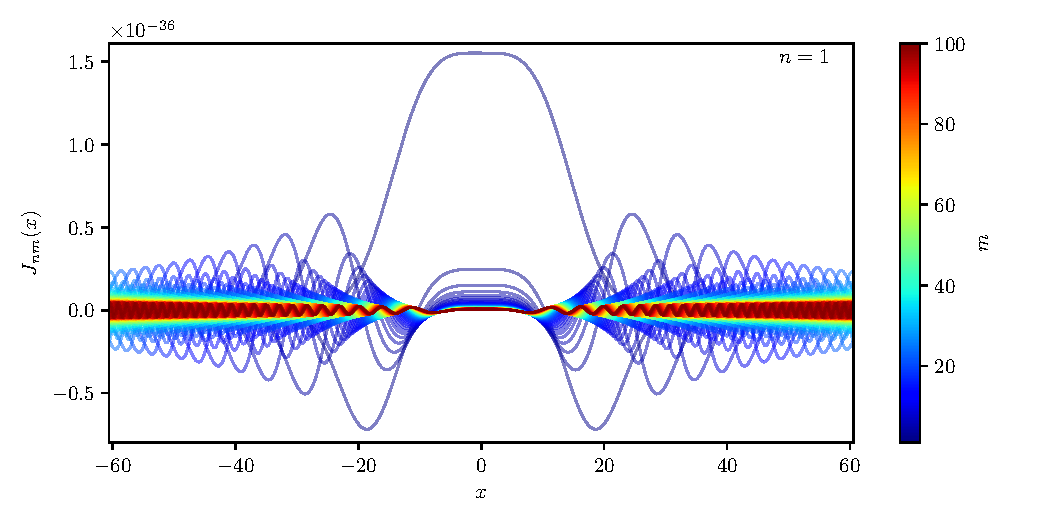
\includegraphics{Jsoln_n1_m100.pdf}
    \caption{Eigenfunctions $J_{nm}(x)$ for the lowest-order spatial eigenmode $n=1$, and a range of frequency eigenmodes up to $m=100$. Their oscillatory forms have varying amplitudes which sum to create the final form of the mean intensity. The largest contribution always comes from the ($n=1, m=1$) lowest-order eigenfunction.}
    \label{fig:jsoln}
\end{figure}
A set of eigenfunctions $J_{nm}(\sigma)$ are plotted in Fig. \ref{fig:jsoln} to illustrate their relative scales for different frequency eigenmodes $m$ at a fixed spatial eigenmode $n$. The overall scale of the $J_{nm}(\sigma)$ are set by the factor $E/(kR^3)$ with $E$ arbitrarily set to 1, $k = \tau_0 \sqrt{\pi} \Delta / R$, and $R = 10^{11}$ cm. With this normalization, an eigenfunction has typical size ${\sim} E a / \left(R^2 \Delta \right) = 10^{-37}$. Additional terms add smaller, faster-oscillating components that lead to higher accuracy upon summation with the lower-order terms. The oscillations of various modes must cancel perfectly to recreate the form of the solution in Eq. \ref{eq:Jrsigmat}, so many modes $m$ and $n$ are required for convergence to the correct solution. Too few (or imprecisely-calculated) modes creates ``ringing'' in the function that indicates the presence of imperfect cancellations in the positive and negative contributions of individual poles. 
\begin{figure}
    \centering
    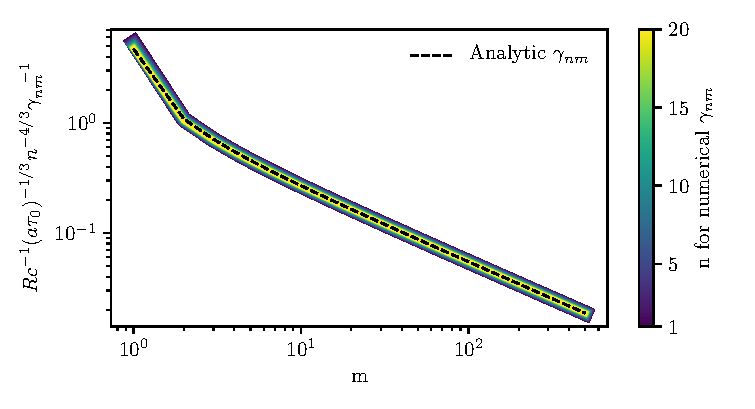
\includegraphics[width=\textwidth]{gamma_nm.pdf}
    \caption{The scaling of numerically-obtained resonant frequencies as compared with the analytic expression in Eq. \ref{eq:gamma_nm}. The data shown is for $\tau_0=10^7$ and $x_s=0.0$.}
    \label{fig:gamma_nm}
\end{figure}
The values of the $\gamma_{nm}$ resonant frequencies can be described approximately with Eq. \ref{eq:gamma_nm}. Their scale depends on $m$, $n$, and the factor $(a\tau_0)^{1/3}$ according to 
\be \label{eq:gamma_nm}
\gamma_{nm} = 2^{-1/3} \pi^{13/6} n^{4/3}\left(m-\frac{7}{8}\right)^{2/3}\frac{c}{R}(a\tau_0)^{-1/3} 
\ee
The size of additional eigenfrequencies scales as a powerlaw in $m$, yet as is seen in Fig. \ref{fig:gamma_nm} the scaling is weak, requiring up to 500 $m$ to reduce the scale of $\gamma_{nm}^{\ \ -1}$ by two orders of magnitude. When sweeping through the imaginary frequency domain to find resonances, this expression is used to set the scale of the sweep points to ensure no $\gamma_{nm}$ are missed. The continuity and close agreement with the analytic expression shown in Fig. \ref{fig:gamma_nm} indicate that the sweep routine accurately brackets and refines the locations of resonances.

The form of a single eigenmode $J_{nm}(\sigma)$ is oscillatory out to some turning point, $\sigma_{tp}$, at which point the function becomes evanescent. The location of the turning point can be found by ignoring the delta-function discontinuity at the source frequency $\sigma_s$ in Eq. \ref{eq:diffusion_plugged_in} and re-examining the resulting homogeneous differential equation. We obtain
\be
\frac{d^2J}{d\sigma^2} & = & \left[ \left( \frac{\kappa_n \Delta }{k} \right)^2 - \frac{3\phi \gamma\Delta^2}{ck}\right] J
\ee
where the line profile is approximated as in Eq. \ref{app:rteqn_derivation}\ref{eq:line_profile_wing}. When the coefficient on the right hand side is positive, exponential growth or decay solutions are found (evanescence). This occurs on the line wings. When the coefficient on the right hand side is negative, oscillatory solutions are found (propagation), which occurs near the line core. The boundary between propagation and evanescence occurs at the turning point, given by
\be
\sigma_{tp} & = & \sqrt{\frac{2a}{\pi}}\left( \frac{k \gamma}{ \kappa_n^2 c \Delta} \right)^{3/2}
\ee
Thus, to ensure accuracy in the final sum of Eq. \ref{eq:Jrsigmat}, the bounds of $\sigma$ must be set sufficiently far outside of $\sigma_{tp}$ such that the function is small at the edges. The scale of an $e$-folding in $J_{nm}(\sigma)$ is $k/(\kappa_n \Delta) = \tau_0 / (\sqrt{\pi} n)$, so a grid of $\sigma$ is chosen that spans a large enough number of $e$-foldings that no oscillatory behavior is present at the boundaries of the calculation.

\subsection{Comparison with Steady State and Monte Carlo}

Integrating $dE/dt d\nu$ from Eq. \ref{eq:dEdtdnu} over all times should give a distribution for the emitted frequencies. It is expected that this time-integrated spectrum of the response to an impulse will agree well with the solution for the $H_0$ steady-state spectrum (Eq. \ref{eq:H0surf}). Dividing by the energy $E$, we find the probability distribution
\be \label{eq:spectrum}
P(\nu) & = &  \frac{16\pi^2 R}{3k\phi E}  \sum_{nm} (-1)^n \gamma_{nm}^{-1} J_{nm}(\sigma).
\ee
Integrating over $\nu$ gives unity according to the sum rule in Eq. \ref{eq:sumrule}. In Fig. \ref{fig:steadystate}, the resulting spectrum is shown for a sum up to $n=20$ and $m=500$ (labelled ``Time-integrated'') as compared with two analytic solutions: the steady-state $J=0$ solution with no time dependence (``Steady State'') and the result for summing \textit{only} spatial modes in the eigenfunction expansion with the time dependence ignored (``Partial Sum''), as in Eq. \ref{eq:H0surf_sum}. This graphic illustrates the physics modeled by each variable in the expansion. For example, the spatial modes contribute to the solutions' accuracy in the core of the line. If more spatial modes were calculated, the agreement between the lines extends further into the core. If additional frequency modes are calculated, faster-oscillating terms are incorporated into the sum over the imaginary frequency variable $\gamma$ which create more perfect cancellations with the lower-order terms, reducing the ``ringing'' seen in the time-integrated spectrum. Extending the calculation deep into the line core by adding additional spatial modes could have an impact on the accuracy of the escape time distribution, but this would only affect the distribution at late times since core photons are trapped for a longer duration before escaping. This was the motivation for choosing a comparatively low number of spatial eigenmodes with respect to the number of frequency eigenmodes calculated. As a result of this choice, we expect that our semianalytic approach will underestimate the number of escaping photon at late times as compared with the Monte Carlo.

\begin{figure}
    \centering
    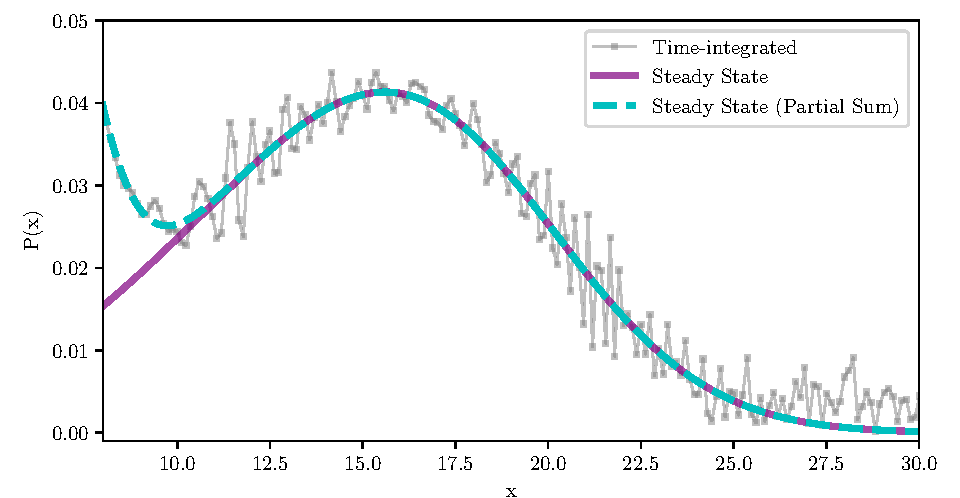
\includegraphics{steadystate.pdf}
    \caption{Comparison of steady-state and time-integrated spectra for 20 spatial eigenmodes and 500 frequency eigenmodes at a line center optical depth of $\tau_0=10^7$. The accuracy of the time-integrated solution is limited by the number of frequency eigenmodes summed. The accuracy of the core behavior for both the partial sum and the time-integrated solution is limited by the number of spatial eigenmodes summed, which is why both solutions fail in the core.}
    \label{fig:steadystate}
\end{figure}

The distribution of the times it takes each photon to escape the sphere is calculated from Eq. \ref{eq:dEdtdnu} by integrating over all frequencies. We obtain
\be
P(t)  & = & \sqrt{\frac{3}{2}} \frac{16\pi^2 R \Delta^2 }{3kE}     \sum_{nm} (-1)^n  e^{-\gamma_{nm}t} \int d\sigma J_{nm}(\sigma) 
\nonumber \\ & = &  \sum_{nm} P_{nm} \gamma_{nm} e^{-\gamma_{nm}t},
\label{eq:waittime}
\ee
which is also normalized to unity. For a sufficient number of spatial modes $n$ and frequency modes $m$, this sum approaches the ``true'' distribution of photon escape times as modeled by Monte Carlo simulations.

The eigenfunction expansion method is an effective characterization of the time-to-escape, yet not a fast enough computational method to use as a distribution for sampling. However, the behavior of the solution is well-understood since the late-time distribution is simply an exponential falloff in photon escape probability. The rate constant of the function is the lowest-order eigenfrequency, $\gamma_{00}$, and its scale is determined by the coefficient $P_{00}$ as in Eq. \ref{eq:pnmsoln}. Thus, an approximate ``fitting function'' that captures both the peak of the escape time distribution and the exponential falloff is
\be \label{eq:fitting_function}
P(t) = \exp{\left[-\left(\frac{t_{\rm diff}}{t}\right)^2\right]} \times \gamma_{00} P_{00} e^{-\gamma_{00}t}.
\ee
The first term represents the early-time distribution, which then transitions to an exponential falloff past a point $ct/R = ct_{\rm diff}/R = (a\tau_0)^{1/3}$, where $t_{\rm diff}$ is a characteristic diffusion timescale. This is shown in Fig. \ref{fig:escape_time} for two different line center optical depths. It is seen that the fitting function matches well with the late-time behavior of the eigenfunction solution, indicating that the tail of the escape time distribution can be modeled effectively by simple exponential decay. The remaining discrepancy between the tail of the distribution and the Monte Carlo data is due to core scattering, which is not accurately modeled by the eigenfunction solution. A cumulative distribution function can be created from Eq. \ref{eq:fitting_function} using a simple rejection method, which allows the function to be sampled rapidly.

\begin{figure}
    \centering
    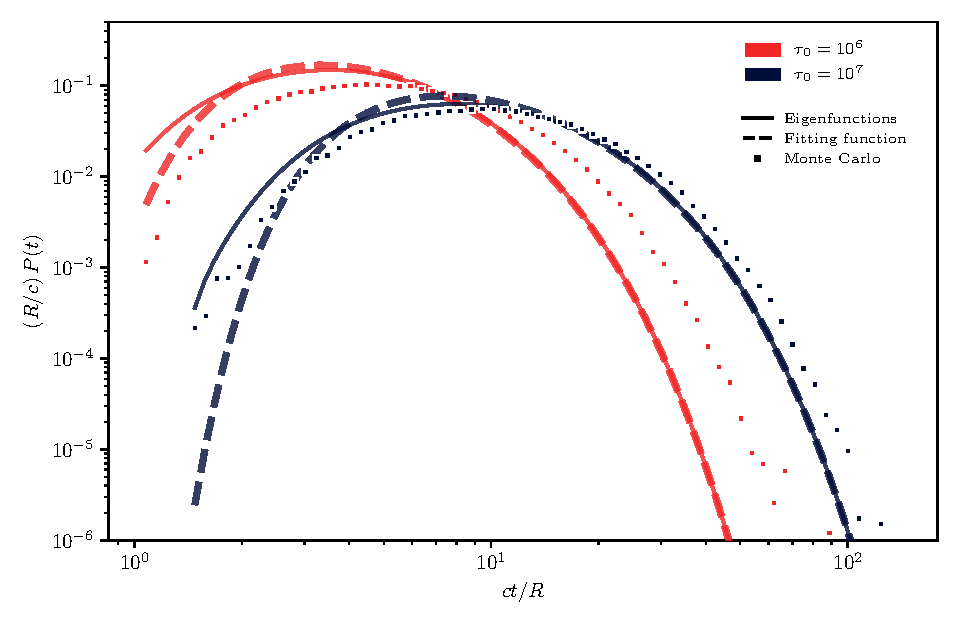
\includegraphics{waittime.pdf}
    \caption{A wait time distribution of escaping photons for two different line center optical depths $\tau_0$, which is fit using Eq. \ref{eq:fitting_function}. A sum over 20 spatial eigenmodes and 500 frequency eigenmodes is labeled ``Eigenfunctions''. All calculations were performed with a monochromatic source of photons at line center ($x_s = 0.0$).}
    \label{fig:escape_time}
\end{figure}

The effect of many scatterings in the Doppler core affects the tail of the escape-time distribution, since photons that become trapped here will take much longer to escape on average. This explains the deficit of photons in the semi-analytic escape time distributions at late times, i.e., the rate constant for the exponential falloff is overestimated slightly as compared with the Monte Carlo. The error in this rate constant is a function of line center optical depth, since the effect from the Doppler core is greatest when it extends into the area of the spectrum where photons most readily escape. In Fig. \ref{fig:tau_scaling}, it is shown that the rate constant of exponential decay converges with the lowest-order eigenfrequency $\gamma_{00}$ at sufficiently high optical depths, following a $t\propto(a\tau_0)^{1/3}$ scaling. At lower optical depths $\tau_0$, the effects of core scattering are most important, leading to a larger discrepancy in the characteristic escape timescale. Here, the Monte Carlo accurately characterizes the photons which scatter in the core many times before escaping, while the semi-analytic solution does not capture this behavior as it uses only the Lorentzian piece of the line profile and does not use enough spatial modes to accurately model the frequency regime near line center. However, as the optical depth grows, the effect of core scattering becomes smaller and the approximations hold much better, agreeing well with the expected analytic scaling for the rate constant.

\begin{figure}
    \centering
    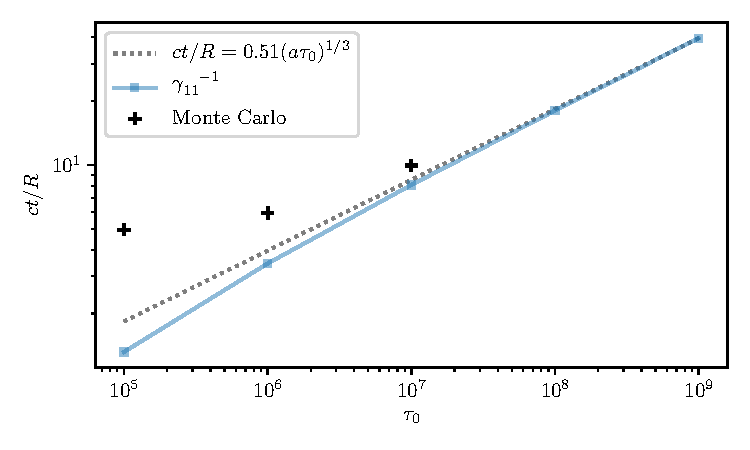
\includegraphics[width=0.75\textwidth]{tau_scaling.pdf}
    \caption{Characteristic timescales as a function of optical depth. The reciprocal of the lowest-order eigenfrequency, $\gamma_{00}$, and a fit of the exponential falloff for the Monte Carlo data are shown to converge to a $t \propto (a\tau_0)^{1/3}$ scaling at large optical depths. The Monte Carlo points on this figure are obtained by fitting only the exponential piece of the escape time distribution to obtain the rate constant.}
    \label{fig:tau_scaling}
\end{figure}


\subsection{Emission Away From Line Center}

\section{Discussion}
% How can you apply the solution? Talk about it as an application of the problem that justifies going through the effort of implementing it. It reads like an introduction right now, but we can modify it to include less detail.
% Don't explain exactly what hybrid diffusion models are. Remove that paragraph. Put a ref in for Smith and Densmore - lot of applications to speed up lya, including core skipping & hybrid diffusion methods. Another method that's been widely applied is modified random walk methods, but htose require a solution of transfer in a sphere. So, the primary application of this calcuation is to develop that random walk model that will be used in future applicaitons. Keep reference to Ahn et al, since they did basically this but not in spherical symmetry.
% Discussion section: tlak about the differences between what we find and the other results from other papers. Add this as well. 
% First part of discussion - compare to previous work and summarize differences. Move some of the comparison with Dijkstra to the discussion.
% Second part - application of solution

Models of heating and escape of hydrogen gas in exoplanet atmospheres can be constructed with an accurate treatment of resonant scattering of \lya in spherical geometry. The Monte Carlo method can be used for this problem, but requires a solution of radiative transfer in a sphere and is limited by its high computational demand for large optical depths where there are many photon scatterings before escape. The primary goal of this work is to present a solution for mean intensity ($J$) and flux ($H = F/4\pi$) of photons near line-center frequency $\nu_0$ in a uniform sphere. We have generalized a solution derived by \cite{2006ApJ...649...14D} (called $H_0$ here) to allow a monochromatic source of photons with frequencies away from line center, and we have made a correction to the incorrect $J=0$ surface boundary condition. This correction allows the proper condition $J=\sqrt{3}H$ to be satisfied, and comes from the introduction of the terms $J_{\rm bc}$ and $H_{\rm bc}$ which are solved using a continuous Fourier expansion in frequency. Enforcement of the correct boundary term leads naturally to expansion of the spatial dependence in terms of spherical Bessel functions. In practice, the continuous expansions are discretized and the Fourier coefficients solved for via a matrix equation. The resulting flux correction, $H_{\rm bc}$, scales as $(a\tau_0)^{-1/3}$ where $a$ is the damping parameter and $\tau_0$ is the line-center optical depth. Thus, for very large optical depths, only a small correction to $H_0$ is needed, while larger errors are present in calculations performed at lower optical depths. Since the Laplacian form of the differential equation is only attainable by approximating the line profile as $\phi \approx a/(\pi x^2)$, these solutions are invalid in areas where the Doppler core of the \lya line has a significant effect on the scattering of photons. The peak of the spectral energy distribution of escaping photons is $x_0 = (a\tau_0)^{1/3}$; as such, calculations performed at low optical depths are likely to be inaccurate due to the close proximity of the spectral peak and the Doppler core of the line profile. By comparison with Monte Carlo simulations, we have shown that the enforcement of the correct frequency-dependent boundary conditions improves the accuracy of these analytic solutions %and correctly tracks changes in the spectrum of escaping photons as the monochromatic source frequency $x_s$ is altered, 
provided a sufficiently large optical depth $\tau_0$. Specifically, this solution shows improvement over previous solutions that utilized a $J=0$ surface boundary condition, such as \cite{1973MNRAS.162...43H}, \cite{1990ApJ...350..216N}, \cite{2006ApJ...649...14D} and others. The surface boundary condition correction $H_{\rm bc}$ is positive in the line wing and negative at the peak of the spectrum, which suggests the previously cited solutions are too large at the spectral peaks and too small further out in the wing, where the error scales approximately as $(a\tau_0)^{-1/3}$. This appears to be the consequence of not enforcing the correct frequency-dependent boundary conditions at the surface of the medium.

Additionally, the time-dependence of the problem is solved under a $J=0$ boundary condition to characterize the distribution of photon escape times. The differential equation cannot be solved except with a semi-analytic approach, utilizing an expansion in both space and photon frequency. By matching boundary conditions on either side of the photon source frequency $x_s$, the flux at the surface of the sphere is found as a function of $t$ and $\nu$, expressed as a sum over many eigenmodes $n$ and $m$---spatial and frequency modes, respectively. Calculating additional spatial eigenmodes provides a more accurate model of the physics nearer to line center, but convergence is slow due to each eigenmode's weak dependence on $n$. Additional frequency eigenmodes introduce fast-oscillating terms that improve the accuracy of the sum, as their contributions cancel with components of lower-order terms to better represent the true solution. Integrating the solution over time produces a spectrum that is shown to agree well with the steady-state calculations in Section \ref{sec:steadystate}, provided a sufficient number of terms in the sum. Integrating the solution over frequency leads to a distribution of photon escape times, which can be compared directly with Monte Carlo simulations. The sum over eigenmodes produces an escape-time distribution that broadly captures the behavior shown by Monte Carlo data---a rise at early times, transitioning to exponential decay in the tail of the distribution. It is expected that the accuracy of the rate constant for the tail of the distribution is limited by the number of spatial terms included in the sum over eigenmodes, as the Doppler core can trap photons at high optical depths until they diffuse outward in frequency, biasing the distribution toward later times. This physics is not modeled by our solution for two reasons: 1) our calculations ignored the Gaussian component of the Voigt line profile, leaving the Lorentzian piece which is accurate only in the line wing, and 2) knowing the core is not modeled accurately, we do not include a large enough number of spatial eigenmodes in the sum to resolve it. However, a fitting function dependent on parameters $a$ and $\tau_0$ is found that adequately represents the escape time distribution within these constraints. The cumulative distribution function could be calculated using a rejection method, which would then be used to sample photon escape times directly rather than computing their travel times by the Monte Carlo method.

This leads in to the primary application of this work: to develop a computationally efficient random walk model in spherical geometry. There are several methods that are commonly used to accelerate Monte Carlo radiation transfer calculations, including core skipping methods \citep{1968ApJ...153..783A,2002ApJ...567..922A} and hybrid diffusion methods \citep{2018MNRAS.479.2065S}. Another approach with wide application is modified random walk methods, such as those discussed in \citet{2002ApJ...567..922A,2015MNRAS.449.4336S} in which Monte Carlo code acceleration is performed for large optical depths in a uniform plane-parallel medium with no absorption. These calculations would need to be generalized to spherical symmetry in order to construct a models of resonant scattering in exoplanet atmospheres as discussed in Section \ref{sec:intro}. The underlying principle is the same, however: an outgoing photon is randomly sampled on the surface of the outgoing sphere by drawing its properties from distributions in outgoing frequencies, directions and escape times, based on solutions to the diffusion equation. A method similar to this has been applied by \citet{2006ApJ...645..792T} to Lyman $\alpha$ transfer using the \cite{1990ApJ...350..216N} solution, but this solution of course does not use the correct frequency-dependent boundary condition at the surface of the sphere. Furthermore, to perform a full radiation hydrodynamic simulation with Monte Carlo acceleration, it will be necessary to calculate radiation forces due to \lya transfer on the faces of each grid cell in the simulation. Similar calculations have been done in \citet{1976ApJ...208..286W} in plane-parallel geometry. However, these solutions are limited to optical depths below $2.5 \times 10^3$. For this work, it would be necessary to model line center optical depths of up to 1 million or more. Such considerations will be taken in future work while developing this solution into a 1D hydrodynamic simulation using radiation forces from accelerated Monte Carlo \lya transfer.

\section{Summary}

We have examined previous solutions to \lya transfer in the limit of large optical depth, noting that the separation of variables and treatment of the boundary condition in \cite{1973MNRAS.162...43H}, \cite{1990ApJ...350..216N}, \cite{2006ApJ...649...14D} and others does not produce a valid solution to the transfer equation. Here, we have derived the solution in spherical geometry with an appropriate treatment of the surface boundary condition as a frequency-dependent quantity, examining the spectral and time dependence of the resulting equations. The key result is that the errors in the previously-cited works have been quantified via a corrective boundary term, $H_{\rm bc}$, which resolves an excess in flux at the spectral peak and a deficit in the line wing of the calculated spectrum of \lya radiation as compared with Monte Carlo. The size of $H_{\rm bc}$ diminishes at larger optical depths, following a predictable $(a\tau_0)^{-1/3}$ scaling. Introducing time-dependence back into the transfer equation leads to another solution which is obtained with a discretized eigenfunction expansion and solved numerically. We demonstrate that it agrees with the steady-state result when integrated over time, though its rate of numerical convergence is quite slow and requires a sum over many modes to become accurate. The time-dependent solution is utilized to create wait-time distributions for photons escaping the sphere of optically-thick hydrogen gas, which can be sampled in lieu of direct Monte Carlo simulations that would ordinarily be computationally demanding. We compare the calculations from the time-dependent solution with Monte Carlo for a sample of line-center optical depths, noting general agreement in the resulting escape time distributions. In future work, these distributions will be fitted and used to accelerate Monte Carlo \lya transfer at large optical depths with potential applications in radiation hydrodynamic simulations of the atmospheres of exoplanets.

\acknowledgments

\appendix
\restartappendixnumbering
\section{ derivation of the transfer equation } \label{app:rteqn_derivation}

The problem is as follows. The radiative intensity $I = dE/(dA dt d\Omega d\nu)$ is the energy per perpendicular area $dA$, per time $dt$, per solid angle $d\Omega$ and per frequency $d\nu$ \citep{1986rpa..book.....R}. Here the time-dependence of $I$ has been ignored, which assumes the fluid is changing on timescales long compared to a light-crossing time. The intensity $I=I(\vec{x},\vec{n}, \nu)$ will be considered a function of position $\vec{x}$, photon (unit) direction vector $\vec{n}$, and cyclic frequency $\nu$. In the Eddington and two-stream approximations, $I(\vec{x},\nu) \simeq J(\vec{x},\nu) + 3 \vec{n} \cdot \vec{H}(\vec{x},\nu)$, where $J=(1/4\pi) \int d\Omega I$ is the mean intensity and $\vec{F} = 4\pi \vec{H}= \int d\Omega \vec{n} I$ is the flux.  

Photons of frequency $\nu$ near line center frequency $\nu_0$ are considered. The Doppler width will be written $\Delta = \nu_0 v_{\rm th}/c$, where $v_{\rm th}=\sqrt{2k_{\rm B}T/m_{\rm H}}$ is the thermal speed of hydrogen atoms of mass $m_{\rm H}$ and temperature $T$, and $c$ is the speed of light. The photon frequency in Doppler units will be written $x = (\nu-\nu_0)/\Delta$. For upper-state de-excitation rate $\Gamma$, the ratio of natural to Doppler broadening is $a=\Gamma/(4\pi \Delta)$. 
The transfer equation is \citep{1986rpa..book.....R}
\be
\frac{1}{c} \frac{\partial I}{\partial t} + \vec{n} \cdot \grad I & =& - \left( \alpha_{\rm sc} + \alpha_{\rm abs} \right) I + (1-p) j_{\rm sc} + j_{\rm em}.
\label{eq:rteqn}
\ee
The scattering coefficient, or inverse mean free path to scattering, is 
\be
\alpha_{\rm sc} & = & n_{\rm sc}\, \frac{\pi e^2}{m_e c}\, f\, \frac{\mathcal{H}(x,a)}{\sqrt{\pi} \Delta}
= k \phi   
\ee
where $n_{\rm sc}$ is the number density of scatterers, $e$ and $m_e$ are the charge and mass of the electron, $f$ is the oscillator strength of the transition, $\mathcal{H}(x,a)$ is the Voigt function, $k = n_{\rm sc} (\pi e^2/m_e c) f$, and the Voigt line profile is $\phi = \mathcal{H}(x,a)/(\sqrt{\pi} \Delta)$, which is normalized as $\int d\nu\, \phi(\nu) = 1$. The absorption coefficient $\alpha_{\rm abs}$, or inverse mean free path to true absorption, is a sum over number density of the absorber times absorption cross section. Once the incoming photon has promoted the electron to an excited state, the collisional de-excitation probability is $p$, and hence only a fraction $1-p$ of the excitations lead to re-emission of photons. Photon destruction will not be considered, so $p$ is set to 0 in this work.

\citet{1973MNRAS.162...43H} first showed that the transfer equation for the mean  intensity $J$ will satisfy a Poisson equation involving second derivatives of space and frequency variables. In this section we will briefly review the derivation of this equation including photon destruction terms and an emission term.

 ``Hummer Case II-b"  \citep{1962MNRAS.125...21H} will be used for the redistribution function, for which the incoming photon is absorbed by the atom according to the natural broadening in the rest frame, re-emitted with a dipole phase function $g(\vec{n},\vec{n}^\prime)=(3/16\pi)(1+[\vec{n}\cdot \vec{n}^\prime]^2)$, which is appropriate for a 1s-2p transition \citep{1982qe}, and the result is averaged over a Maxwell-Boltzmann distribution of speeds for the atom. The result can be written
\be
j_{\rm sc}(\vec{x},\vec{n},\nu) & = & k \int \frac{ d^3v}{ \pi^{3/2} v_{\rm th}^3} e^{-v^2/v_{\rm th}^2}\, 
\int d\Omega^\prime \int d\nu^\prime \,
g(\vec{n},\vec{n}^\prime) 
\nonumber \\ & \times & 
\delta \left( \nu - \nu^\prime - \nu_0 \vec{v} \cdot (\vec{n}-\vec{n}^\prime)/c \right)
\left( \frac{\Gamma/4\pi^2}{ \left(\nu^\prime - \nu_0 - \nu_0 \vec{v} \cdot \vec{n}^\prime/c \right)^2 + (\Gamma/4\pi)^2 } \right)  \,
I(\vec{x},\vec{n}^\prime,\nu^\prime)
\nonumber \\ & = & 4\pi k \int d\Omega^\prime \int d\nu^\prime R(\vec{n},\nu; \vec{n}^\prime,\nu^\prime) I(\vec{x},\vec{n}^\prime,\nu^\prime),
\ee
which defines the Case II-b redistribution function
\be
R(\vec{n},\nu; \vec{n}^\prime,\nu^\prime) & = & \frac{ g(\vec{n},\vec{n}^\prime) }{ 4\pi }
\int \frac{ d^3v}{ \pi^{3/2} v_{\rm th}^3} e^{-v^2/v_{\rm th}^2}\,
\delta \left( \nu - \nu^\prime - \nu_0 \vec{v} \cdot (\vec{n}-\vec{n}^\prime)/c \right)
\left( \frac{\Gamma/4\pi^2}{ \left(\nu^\prime - \nu_0 - \nu_0 \vec{v} \cdot \vec{n}^\prime/c \right)^2 + (\Gamma/4\pi)^2 } \right)
\ee
found in \citet{1962MNRAS.125...21H}.


The integral of the redistribution function over outgoing and incoming frequency are
\be
\int d\nu\ R(\vec{n},\nu; \vec{n}^\prime,\nu^\prime) 
& = & \frac{1}{4\pi} g(\vec{n},\vec{n}^\prime) \phi(\nu^\prime)
\ee 
and
\be
\int d\nu^\prime \ R(\vec{n},\nu; \vec{n}^\prime,\nu^\prime) 
& = & \frac{1}{4\pi} g(\vec{n},\vec{n}^\prime) \phi(\nu)
\ee 
where the right hand side is the usual Voigt function, the thermal average of the Lorentzian. The former result implies that the integrated source and sink terms for scattering cancel for $p=1$. In addition, $d\nu d\Omega 4\pi R(\vec{n},\nu; \vec{n}^\prime,\nu^\prime)/\phi(\nu^\prime) $ is the normalized distribution for the outgoing $\vec{n}$ and $\nu$ given the incoming $\vec{n}^\prime$ and $\nu^\prime$. 

This probability distribution can be used to define the moments of the frequency shift
\be
\langle \Delta \nu^n \rangle & = & \frac{ \int d\nu^\prime R (\nu-\nu^\prime)^n}{\int d\nu^\prime R}
= \frac{1}{\phi(\nu)}
\int \frac{ d^3v}{ \pi^{3/2} v_{\rm th}^3} e^{-v^2/v_{\rm th}^2}\,
\left( \frac{\nu_0 \vec{v} \cdot (\vec{n}-\vec{n}^\prime) }{c} \right)^n
\left( \frac{\Gamma/4\pi^2}{ \left(\nu - \nu_0 - \nu_0 \vec{v} \cdot \vec{n}/c \right)^2 + (\Gamma/4\pi)^2 } \right),
\ee
which are functions of $\nu$, $\vec{n}$ and $\vec{n}^\prime$. These integrals can be evaluated in terms of the dimensionless moments of the parallel velocity distribution, defined as
\be
\langle u_\parallel^n \rangle(x,a) & = & \frac{a/\pi }{\mathcal{H}(x,a)} \int 
\frac{du_\parallel u_\parallel^n e^{-u_\parallel^2}  }{(x-u_\parallel)^2 + a^2}.
\ee
The end results for the first and second moments are
\be
\langle \Delta \nu \rangle & = & \Delta \langle u_\parallel \rangle \left( 1 - \vec{n} \cdot \vec{n}^\prime \right)
\\
\langle \Delta \nu^2 \rangle & = & \Delta^2 
\left[ \langle u_\parallel^2 \rangle
\left( 1 - \vec{n} \cdot \vec{n}^\prime \right)^2
+ \frac{1}{2} \left( 1 - \left( \vec{n} \cdot \vec{n}^\prime\right)^2 \right) \right].
\ee

For small frequency shifts $\nu-\nu^\prime$, the incoming intensity may be expanded as 
\be
I(\vec{x},\vec{n}^\prime,\nu^\prime) & \simeq  &
I(\vec{x},\vec{n}^\prime,\nu) 
+ 
\frac{\partial I(\vec{x},\vec{n}^\prime,\nu)}{\partial \nu }(\nu^\prime-\nu)
+ \frac{1}{2} \frac{\partial^2 I(\vec{x},\vec{n}^\prime,\nu)}{\partial \nu^2} (\nu^\prime-\nu)^2 + ...
\ee 
and the Fokker-Planck expansion of $j_{\rm sc}$ is
\be
j_{\rm sc}(\vec{x},\vec{n},\nu) & \simeq  & 4\pi k \int d\Omega^\prime \int d\nu^\prime R(\vec{n},\nu; \vec{n}^\prime,\nu^\prime) 
\left[ 
I(\vec{x},\vec{n}^\prime,\nu) + \frac{\partial I(\vec{x},\vec{n}^\prime,\nu)}{\partial \nu }(\nu^\prime-\nu)
+ \frac{1}{2} \frac{\partial^2 I(\vec{x},\vec{n}^\prime,\nu)}{\partial \nu^2 }(\nu^\prime-\nu)^2
\right]
\nonumber \\ 
& =& 
k\phi(\nu) \int d\Omega^\prime g 
\left[ 
I(\vec{x},\vec{n}^\prime,\nu) 
- \frac{\partial I(\vec{x},\vec{n}^\prime,\nu)}{\partial \nu }
\langle \Delta \nu \rangle
+ \frac{1}{2} \frac{\partial^2 I(\vec{x},\vec{n}^\prime,\nu)}{\partial \nu^2 }
\langle \Delta \nu^2 \rangle
\right]
\ee 
To perform the angular integrals, the Eddington approximation for the angular dependence is inserted with the following result
\be
j_{\rm sc} & = & k\phi J - k\phi \Delta \langle u_\parallel \rangle \left( \frac{\partial J}{\partial \nu} - \frac{6}{5} \vec{n} \cdot \frac{\partial \vec{H}}{\partial \nu} \right)
+ \frac{1}{2} \Delta^2 k\phi \left[ 
\frac{\partial^2 J}{\partial \nu^2} \left( \frac{7}{5} \langle u_\parallel^2 \rangle + \frac{3}{10} \right)
- \frac{12}{5} \langle u_\parallel^2 \rangle 
\vec{n} \cdot \frac{\partial^2 \vec{H}}{\partial \nu^2} \right]
\nonumber \\ & \simeq & 
k\phi J - k\phi \Delta \langle u_\parallel \rangle  \frac{\partial J}{\partial \nu} 
+ \frac{1}{2} \Delta^2 k\phi \left( \frac{7}{5} \langle u_\parallel^2 \rangle + \frac{3}{10} \right)
\frac{\partial^2 J}{\partial \nu^2} .
\label{eq:jsc}
\ee
The first term in Eq. \ref{eq:jsc}, $k\phi J$, represents re-emission of the photon through de-excitation of the atom. It cancels the $-k\phi J$ term in Eq. \ref{eq:rteqn} that corresponds to excitation of the atom. The terms involving frequency derivatives of $\vec{H}$, if carried through the calculation,end up giving terms smaller than then largest terms by a factor of $1/x^2$, which is small on the line wing. These terms are ignored from here on.

If only scattering is included, the transfer equation becomes
\be
\frac{1}{c} \frac{\partial }{\partial t} \left( J + 3\vec{n} \cdot \vec{H} \right)
+ \vec{n} \cdot \grad \left( J + 3\vec{n} \cdot \vec{H} \right)
& = & - k\phi \Delta \langle u_\parallel \rangle  \frac{\partial J}{\partial \nu} 
+ \frac{1}{2} \Delta^2 k\phi \left( \frac{7}{5} \langle u_\parallel^2 \rangle + \frac{3}{10} \right)
\frac{\partial^2 J}{\partial \nu^2}.
\ee
Integrating over angle and frequency then gives
\be
\frac{1}{c} \frac{\partial J(\vec{x}) }{\partial t} +  \grad \cdot \vec{H}(\vec{x}) & = & \int d\nu
\left( - k\phi \Delta \langle u_\parallel \rangle  \frac{\partial J}{\partial \nu} 
+ \frac{1}{2} \Delta^2 k\phi \left( \frac{7}{5} \langle u_\parallel^2 \rangle + \frac{3}{10} \right)
\frac{\partial^2 J}{\partial \nu^2}
\right) 
\nonumber \\ & =& 
k \int d\nu J \frac{\partial }{\partial \nu} 
\left( \phi \Delta \langle u_\parallel \rangle
+ \frac{\partial }{\partial \nu}\left[ \frac{1}{2} \phi \Delta^2 
\left( \frac{7}{5} \langle u_\parallel^2 \rangle + \frac{3}{10}  \right) \right]
\right) = 0,
\ee
where $\vec{H}(\vec{x})$ is the frequency integrated flux, and $\grad \cdot \vec{H}(\vec{x})  = 0 $ if there are no sources or sinks of radiation. Integration by parts has been used to factor $J$ out, assuming each term goes to zero at infinity. The quantity inside brackets must be constant, and since each term should go to zero at infinity, that constant is zero. Hence the first and second moments of the frequency shift are related by
\be
\phi \Delta \langle u_\parallel \rangle
& = & -  \frac{\partial }{\partial \nu}\left[ \frac{1}{2} \phi \Delta^2 
\left( \frac{7}{5} \langle u_\parallel^2 \rangle + \frac{3}{10}  \right) 
\right].
\ee
As an example, on the damping wing, the line profile can be approximated as 
\be \label{eq:line_profile_wing}
\phi \simeq \frac{a}{\pi x^2}
\ee
with $\langle u_\parallel \rangle \simeq 1/x$ and $\langle u_\parallel^2 \rangle \simeq 1/2$, and so this identity is satisfied. The redistribution function can then be rewritten
\be
j_{\rm sc} & \simeq & k\phi J + \frac{1}{2} k \Delta^2 \frac{\partial }{\partial \nu} 
\left[ \phi  \left( \frac{7}{5} \langle u_\parallel^2 \rangle + \frac{3}{10}  \right)\frac{\partial J}{\partial \nu}  \right]
\simeq k\phi J + \frac{1}{2} k \Delta^2 \frac{\partial }{\partial \nu} 
\left( \phi \frac{\partial J}{\partial \nu}  \right)
\ee
where the last equality (see e.g. \citealt{1994ApJ...427..603R}) is valid on the damping wing where $\langle u_\parallel^2 \rangle \simeq 1/2$.
The following equations will use the approximations for the damping wing.

Thus far the transfer equation is
\be
\frac{1}{c} \frac{\partial }{\partial t} \left( J + 3\vec{n} \cdot \vec{H} \right) + \vec{n} \cdot \grad \left( J + 3 \vec{n} \cdot \vec{H} \right)
& =& j_{\rm em}
- \left( k\phi + \alpha_{\rm abs} \right) \left( J + 3 \vec{n} \cdot \vec{H} \right)
+
(1-p) \left[
k\phi J + \frac{1}{2} k \Delta^2 \frac{\partial }{\partial \nu} 
\left( \phi \frac{\partial J}{\partial \nu}  \right)
\right]
\nonumber \\ & \simeq & 
j_{\rm em} - 3k\phi \vec{n} \cdot \vec{H} - \left( p k\phi  + \alpha_{\rm abs} \right) J 
+ \frac{1}{2} k \Delta^2 \frac{\partial }{\partial \nu} 
\left( \phi \frac{\partial J}{\partial \nu}  \right),
\label{eq:rteqn2}
\ee
where leading order dissipative terms were kept in the second equality.
The moment equations are
\be
\frac{1}{c} \frac{\partial J}{\partial t} + \grad \cdot \vec{H} & = & j_{\rm em} 
- \left(p k\phi +  \alpha_{\rm abs} \right) J
+ \frac{1}{2} k \Delta^2 \frac{\partial }{\partial \nu} 
\left( \phi \frac{\partial J}{\partial \nu}  \right)
\ee
and
\be
\frac{1}{c} \frac{\partial \vec{H}}{\partial t} + \frac{1}{3} \grad J & =& - \left( k \phi + \alpha_{\rm abs} \right) \vec{H}.
\ee
The $\partial \vec{H}/\partial t$ term may be dropped for slowly changing sources.
Assuming the coefficients are constant in space, these two equations can be combined together to find
\be
\frac{1}{c} \frac{\partial J}{\partial t} - \frac{1}{3 (k\phi + \alpha_{\rm abs})} \nabla^2 J
& =& j_{\rm em} 
- \left( p k\phi +  \alpha_{\rm abs} \right) J
+ \frac{1}{2} k \Delta^2 \frac{\partial }{\partial \nu} 
\left( \phi \frac{\partial J}{\partial \nu}  \right).
\ee
Making the change of variables to $d\sigma$ using
\be \label{eq:change_of_variables}
d\sigma = \sqrt{\frac{2}{3}}\frac{d\nu}{\phi \Delta^2},
\ee
the equation can be rewritten in the standard form \citep{1973MNRAS.162...43H}
\be
-3 \left( \frac{k\phi + \alpha_{\rm abs}}{c}\right) \frac{\partial J}{\partial t} + \nabla^2 J + \left( \frac{k}{\Delta} \right)^2 \left( 1 + \frac{\alpha_{\rm abs}}{k\phi} \right)\frac{\partial^2 J}{\partial \sigma^2} & = & 
-3 \left( k\phi + \alpha_{\rm abs}\right) j_{\rm em}
+ 3 \left( k\phi + \alpha_{\rm abs}\right) \left( pk\phi + \alpha_{\rm abs}\right) J.
\label{eq:finaleqn}
\ee
    
For emission with luminosity $L$, with a delta function in space $\delta^3(\vec{x} - \vec{x}_s)$ at source position $\vec{x}_s$, a delta function in frequency $\delta(\nu-\nu_{\rm s})$ at source frequency $\nu_{\rm s}$, and isotropic in angles, the emission coefficient is
\be
j_{\rm em} & = & \frac{L}{4\pi} \delta^3(\vec{x} - \vec{x}_s) \delta(\nu-\nu_{\rm s}).
\label{eq:jem}
\ee
Multiplying by a factor $-3k\phi$, as appears in Eq. \ref{eq:finaleqn}, the delta function in $\nu$ becomes a delta function in $\sigma$ of the form
\be
-3k\phi j_{\rm em}  &= & - \frac{ \sqrt{6} kL}{4\pi \Delta^2} \delta^3(\vec{x} - \vec{x}_s) \delta (\sigma - \sigma_{\rm s}),
\label{eq:jem_v2}
\ee
where $\sigma_s = \sigma(\nu_s)$. 


\bibliography{ref.bib}{}
\bibliographystyle{aasjournal}



\end{document}

